\chapter{Photoassociation in ultracold gases} \label{ch:chap3}
\section{Introduction} \label{sec:pas_intro}
Recall from Ch.\,\ref{ch:intro} that photoassociation is the process of creating molecular states from colliding free atoms.
This technique tends to create long-range weakly-bound molecules due to the excitation rate depends on the overlap of the initial scattering state and the bound state.
Fig.\,\ref{fig:3pasSch} illustrates the PA process outlined previously and adds schematic wavefunctions.
This highlights that the outer lobe of the wave function makes the largest contribution to the overlap integral, which is situated around the classical turning point of the molecule, $R_c$ \cite{Bohn1999,bav00}.
\begin{figure}
	\centerline{
	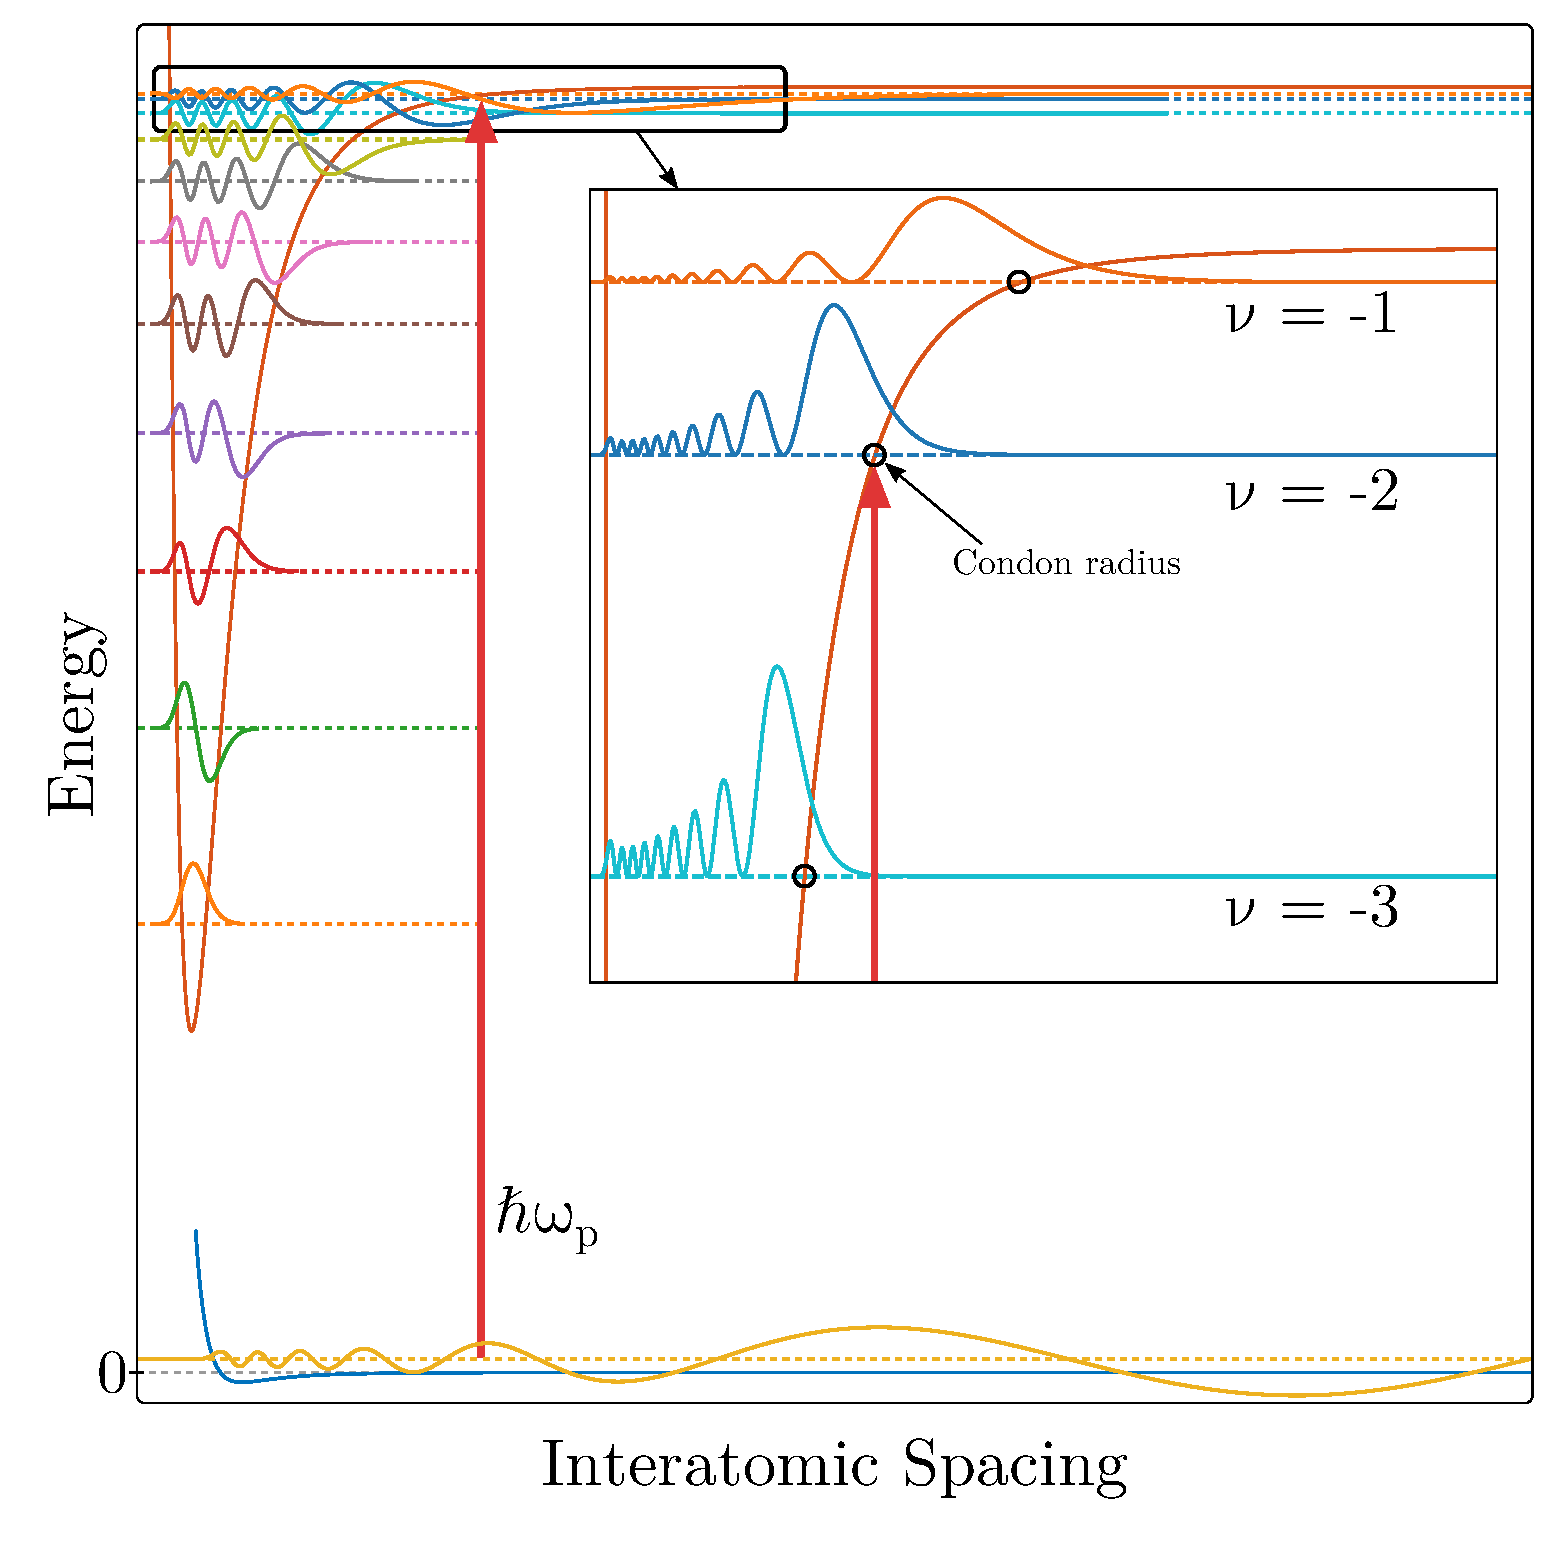
\includegraphics[width=\textwidth]{PASwithWF.pdf}}
	\caption{Schematic of the photoassociation process}{The photoassociation process relies on favorable overlap between the initial free particle state and the final bound state. An example incoming wavefunction at collision energy $\epsilon > 0$ is shown in yellow along the lower potential. This state is then coupled to a vibrationally excited bound-state wavefunction in the upper potential using a photoassociation laser at frequency $\omega_\text{p}$. The inset shows the probability density of the excited states and the classical turning point for each bound state.}
	\label{fig:3pasSch}
\end{figure}
Contribution to the overlap in the region $r < R_c$ is negligible due to the fast oscillations in the interior region of either wavefunction.
Furthermore, the outer lobe moves inward as the binding energy of the bound state molecules is increased. 
This causes a decrease of the overlap with the initial scattering state and consequently a reduction in the rate of molecular formation may be observed \cite{Krems2009a,Julienne2009a,nse06,Jones2006}.
%By comparing the amplitude rhotoassociation is considered a long-range probe used to measure and determine characteristics about the complex short-range potential .

%Fig.\,\ref{fig:3pasSch}b shows an alternative view of photoassociation in the dressed-state picture.
%In this formulation, photoassociation is naturally described by resonant scattering theory whereby bound states are considered embedded in a continuum of thermally distributed scattering states.
%Collisions between atoms are altered by the presence of light-field coupling that may, in general, lead to modification of the elastic scattering between atoms or introduce loss due to inelastic scattering  \cite{Jones2006, Thorsheim1987, Fano1961, Nicholson2015a}.

% Summary
Thus, while a conceptual description of photoassociation as colliding particles associating to a bound-state is straightforward, a rigorous theoretical understanding of the process requires discussion of several fundamental topics related to the behavior of ultracold gases.
In particular, the rate of photoassociation of a trapped gas is sensitive to a number of energetic effects including the distribution of thermal kinetic energy, differences in potential energy due to trapping potentials, and internal interaction energy due to interparticle scattering \cite{Julienne2009a}.
The remainder of this chapter will discuss these considerations and end by formulating analytic descriptions for describing one- and two-photon photoassociation spectra.

\section{Theory of trapped boson gases} \label{sec:trapped_gases}
This section briefly covers the statistical mechanics describing a trapped thermal bosonic gas.
From this description we discuss the evolution of the atomic densities during free expansion and discern how to extract physical parameters of the gas from absorption images.

In the limit of large, fixed particle number and thermal equilibrium, the trapped density distribution $n(\vec{r})$ is given by
\begin{equation} \label{eq:2thermDist}
	n_{th}(\vec{r}) = \int \frac{d\vec{p}}{(2\pi\hbar)^3} \frac{1}{\exp{(E_p(\vec{r}) - \mu)/k_BT} - 1}
\end{equation}
where $E_p(\vec{r}) = \frac{p^2}{2m} + V(\vec{r})$.
This semi-classical description assumes negligible occupation of the trap ground state.
This integral can be evaluated by defining the quantities
\begin{equation*}
	x = \frac{p^2}{2mk_BT} \quad\quad z(\vec{r}) = e^{[\mu - V(\vec{r})]/k_BT} = \xi e^{-V(\vec{r})/k_BT}
\end{equation*}
where $\xi$ is known as the fugacity \cite{psm02}.
After a change of variables from $p$ to the dimensionless quantity $x$, Eq.\,\ref{eq:2thermDist} reduces to
\begin{equation}
	n_{th}(\vec{r}) = \frac{2}{\sqrt{\pi}}\frac{1}{\lambda_T^3}\int dx \frac{\sqrt{x}}{z(\vec{r})^{-1}e^x-1}
\end{equation}
where $\lambda_T = \sqrt{\frac{2 \pi \hbar^2}{m k_B T}}$ is the de Broglie wavelength.
This is a common integral in problems of this type and may be rewritten as \cite{Demarco1998, Ketterle1999, psm02}
\begin{equation}
\begin{split}
	\int_0^{\infty}dx\frac{x^{\gamma-1}}{z^{-1}e^x-1} &= \sum_{n=1}^{\inf}\int_0^{\infty}dx \,x^{\gamma-1}e^{-nx}z^n \\
	&=\Gamma(\gamma)\text{Li}_{\gamma}[z]
\end{split}
\end{equation}
where $\text{Li}_{\gamma}[z]$ is the polylogarithm function defined by $\text{Li}_{\gamma}[z] = \sum_{n=1}^{\inf}\frac{z^n}{n^{\gamma}}$ and $\Gamma(\gamma)$ is the Euler gamma function.
This function is also known as the Bose enhancement function \cite{Ketterle1999} and describes the bunching of bosonic particles near degeneracy.
The thermal distribution is then given by
\begin{equation}
	\begin{split}
	n_{th}(\vec{r}) &= \frac{\Li{\ssfrac{3}{2}}{z(\vec{r})}}{\lambda_T^3} \\
				 &= \frac{1}{\lambda_T^3}\Li{\ssfrac{3}{2}}{\,\xi\,\exp{-V(\vec{r})/k_BT}}
	\end{split}
\end{equation}
For harmonic traps $V(\vec{r}) = \frac{m}{2}\displaystyle\sum_i\omega_i^2r_i^2$ and the \textit{in situ} density profile is
\begin{equation} \label{eq:harmTrapDist}
	n_{th}(\vec{r}) = \frac{1}{\lambda_T^3}\Li{\ssfrac{3}{2}}{\xi \,\exp{\sum_i\frac{-m\omega_i^2r_i^2}{2 k_B T}}}
\end{equation}
In the classical, or high-temperature limit, $\Li{\ssfrac{3}{2}}{z(\vec{r})} \approx z(\vec{r})$ and we recover the classical Maxwell-Boltzmann description \cite{psm02}.
\begin{equation}
	n_{MB}(\vec{r}) = \frac{\xi}{\lambda_T^3}\exp{\sum_i\frac{-m\omega_i^2r_i^2}{2 k_B T}}
\end{equation}

\subsection{Extracting data from column densities} \label{ssec:tof}
This description of thermal bosons in a trapping potential is useful but we must continue a step further and see how Eq.\,\ref{eq:harmTrapDist} evolves when atoms are released from the trap and allowed to expand in free space. 
Once the trapping potential is removed, neglecting any collisions, atoms will follow trajectories according to
\begin{equation}
	\frac{d\vec{r}}{dt}=\frac{\vec{p}}{m} \quad \text{and} \quad \frac{d\vec{p}}{dt}=0
\end{equation}
Thus, an atom measured at position $\vec{r}$ after the time-of-flight, $t$, will have traveled a distance $\brcurs = \frac{\vec{p}t}{m}=\vec{r} - \vec{r}_0$ from its initial position $\vec{r}_0$.
This is shown schematically in Fig.\,\ref{fig:ballisticExp}.
\begin{figure} 
	\centerline{
	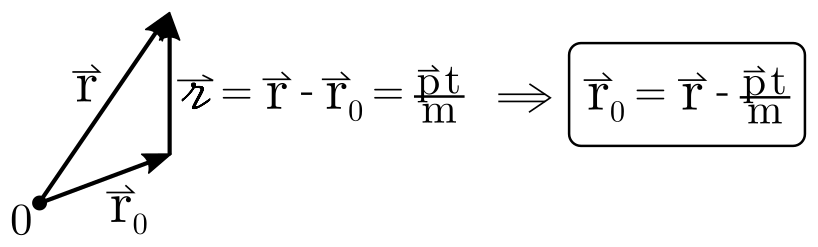
\includegraphics[width=0.7\textwidth]{ballisticExpansion.png}}
	\caption{Ballistic expansion of particles}{Schematic representation particle displacement vectors used to determine how time-of-flight expansion transforms the initial density distribution}
	\label{fig:ballisticExp}
\end{figure}
The spatial density then evolves to
\begin{equation}
\begin{split}
	n_{th}'(\vec{r},t) &= \int \frac{d^3\vec{r}\,d^3\vec{p}}{(2\pi\hbar)^3}\frac{1}{\exp{\left[\frac{p^2}{2m} + V(\vec{r}') - \mu\right]\frac{1}{k_BT}}-1}\delta^3\left(\vec{r}-\frac{\vec{p}t}{m}-\vec{r}'\right) \\
	&= \int \frac{d^3\vec{p}}{(2\pi\hbar)^3}\frac{1}{\exp{\left[\frac{p^2}{2m} + V\left(\vec{r}-\frac{\vec{p}t}{m}\right)) - \mu\right]\frac{1}{k_BT}}-1} 
\end{split}
\end{equation}
where $n_{th}'(\vec{r},t)$ is simply the time-evolved thermal density such that $n_{th}'(\vec{r},t=0) = n_{th}(\vec{r})$.
Adding the harmonic potential, the free expansion after release from a harmonic trap is found to be self-similar and amounts to rescaling the the spatial coordinates \cite{Demarco1998}.
Thus the scaled spatial profile is given by
\begin{equation} \label{eq:thermalFit}
	n_{th}'(\vec{r},t) = \frac{1}{\lambda_T^3} 
\left(\, \prod_{j=1}^3 \frac{1}{1+\omega_j^2 t^2} \right) 
\Li{\ssfrac{3}{2}}{ \xi \, \exp{\sum_{i=1}^3 \frac{-m\omega_i^2r_i^2}{2k_BT} \frac{1}{1+\omega_i^2t^2}} }
\end{equation}

From this description of the spatial distribution after time-of-flight expansion, we may now consider the relation of absorption images to the physical characteristics of the gas.
Absorption imaging is a technique whereby a spatially resolved image of (resonant or near-resonant) laser light is recorded after it has passed through a gas of atoms.
When illuminated, the atomic sample will absorb and scatter photons out of the laser beam resulting in the imprint of the atoms "shadow" on the laser's recorded image.
Then using Beer's law \cite{Foot2005, Hueck2017, Reinaudi2007}, the total absorption of photons may be related to the product of the number density of scattering particles along the optical path and the absorption cross section \cite{Mickelson2010b}. 
This results in a measurement of the "optical depth" of the gas along a column density. 
Notably, this measurement occurs along a particular direction through the gas, which limits our analysis of the gases properties to the two-dimensional plane orthogonal to the laser beam.

Experimentally, the optical depth (OD) is computed by taking the natural logarithm of a ratio of the images obtained from the camera (Sec.\,\ref{sec:absImagingTech}).
This OD may then be fit using the analytic form of the expanded density profile in Eq.\,\ref{eq:thermalFit} to extract physical quantities.
To see this, we equate the OD image to be proportional to the spatial density profile after the time-of-flight expansion integrated along the optical path through the atoms.
\begin{equation} \label{eq:polyLogExp}
\begin{split}
	\text{OD} = \text{ln} \left( \frac{\text{Atom Image}}{\text{Background Image}} \right) &= \sigma_{abs} \int_{-\inf}^{\inf} dz \, n_{th}'(\vec{r},t) \\ 
&= \frac{\sigma_{abs}}{\lambda_T^3} \left( \, \prod_{j=1}^3 \frac{1}{1+\omega_j^2t^2}\right) \int_{-\inf}^{\inf} dz\,\Li{\ssfrac{3}{2}}{\xi \,\exp{\sum_{i=1}^3 \frac{-r_i^2}{2\sigma_i^2}}}
\end{split}
\end{equation}
where $\sigma_i^2 = \frac{k_BT}{m\omega_i^2}(1+\omega_i^2t^2)$ and $\sigma_{\text{abs}}$ is the optical absorption cross section dependent on the imaging laser frequency.

Before proceeding, let us rewrite the polylogarithm in terms of it's series representation and integrate over a single dimension to replicate the column density image of the experimental data.
\begin{equation}
	\int_{-\inf}^{\inf} dz\,\Li{\ssfrac{3}{2}}{\xi \,\exp{\sum_{i=1}^3 \frac{-r_i^2}{2\sigma_i^2}}} = 
	\int_{-\inf}^{\inf} dz\, \sum_{n=1}^{\inf} \frac{\xi^n}{n^{3/2}}\exp{\frac{-x^2}{2\sigma_x^2} - \frac{y^2}{2\sigma_y^2} - \frac{z^2}{2\sigma_z^2}}^n
\end{equation}
Defining $\rho=\exp{\frac{-x^2}{2\sigma_x^2} - \frac{y^2}{2\sigma_y^2}}$ and expanding
\begin{equation} \label{eq:polyFullExp}
	=\int_{-\inf}^{\inf} dz\, \xi\,\rho\,e^{\frac{-z^2}{2\sigma_z^2}} + 
 \frac{\xi^2}{2^{3/2}}\rho^2\,e^{\left(\frac{-z^2}{2\sigma_z^2}\right)^2} + 
 \frac{\xi^3}{3^{3/2}}\rho^3\,e^{\left(\frac{-z^2}{2\sigma_z^2}\right)^3} + \cdots
\end{equation}
This expansion readily shows the dependence on $z$. 
By considering each term separately and integrating each along $z$, we find $\displaystyle\int_{-\inf}^{\inf} dz\, \sum_{n=1}^{\inf}\exp{\frac{-n z^2}{2\sigma_2^2}} = \frac{\sqrt{2\pi}}{n^{1/2}}\sigma_z$ \cite{Ketterle1999, Gotlibovych2014}.
Rewriting Eq.\,\ref{eq:polyFullExp} and using this result
\begingroup
\addtolength{\jot}{1em}
\begin{equation}
\begin{split}
	&=\int_{-\inf}^{\inf} dz\, \sum_{n=1}^{\inf}\frac{\xi^2\rho^n}{n^{3/2}}\,\exp{\frac{-n z^2}{2\sigma_2^2}} \\
	&=\sqrt{2\pi}\sigma_z\underbrace{\sum_{n=1}^{\inf}\frac{\xi^n\rho^n}{n^2}}_{\displaystyle\Li{2}{\xi\,\rho}}
\end{split}
\end{equation}
\endgroup

\noindent Returning to Eq.\,\ref{eq:thermalFit}, the optical depth is given by
\begin{equation}
	OD(x,y) = \frac{\sqrt{2\pi}}{\lambda_T^3} \sigma_{abs} \sigma_z \left( \, \prod_{j=1}^3 \frac{1}{1+\omega_i^2t^2}\right)\Li{2}{\xi\,\exp{\frac{-x^2}{2\sigma_x^2} - \frac{y^2}{2\sigma_y^2}}}
\end{equation}
This equation still has one unknown, $\sigma_z$, that we cannot readily measure.
This is overcome by measuring a specific value of the optical depth, the peak optical depth, $OD_\text{peak}=OD(x=0,y=0)$.
\begin{equation}
	OD_{\text{peak}} = \frac{\sqrt{2\pi}}{\lambda_T^3} \sigma_{abs} \sigma_z \left( \, \prod_{j=1}^3 \frac{1}{1+\omega_i^2t^2}\right)\Li{2}{\xi}
\end{equation}
Thus the relation between the measured optical depth and the spatial density distribution is given by
\begin{equation} \label{eq:OD}
	OD(x,y) = \frac{OD_{\text{peak}}}{\Li{2}{\xi}}\Li{2}{\xi\,\exp{\frac{-x^2}{2\sigma_x^2} - \frac{y^2}{2\sigma_y^2}}}
\end{equation}
with $\sigma_i^2 = \frac{k_BT}{m\omega_i^2}(1+\omega_i^2t^2)$.
In the limit of long expansion time during time-of-flight, namely $t \gg \omega_x^{-1}, \omega_y^{-1}, \omega_z^{-1}$ then the widths approach $\sigma_i^2\rightarrow\frac{k_BT}{m}t^2$.
From this long-time expansion, the atom temperature is given along each axis by
\begin{equation}
	T_i=\frac{m \sigma_i^2}{k_Bt^2}
\end{equation}

In general, the limiting factor for the maximum allowed expansion time is caused by center-of-mass motion of the cloud under the influence of gravity. 
On the Neutral apparatus, we typically utilize drop times $\approx\!30$\,ms before we are no longer able to view the atoms.
For shallow traps, $\omega_i$ on the order of $<\!10$\,Hz, the applicability of the above long-time approximation should be verified before claiming temperatures, as cold atoms may not approach the long-time limit of expansion, $\omega_i^2t^2 \gg 1$, before falling out of frame.

Finally, we determine the total number of atoms in the trapping potential by formally requiring the particle number to be fixed as $n_{th}(\vec{r})\,\Rightarrow\,n_{th}'(\vec{r},t)$.
\begin{equation}
\begin{split}
	N&=\int_{-\inf}^{\inf} d^3\vec{r}\, n_{th}(\vec{r}) = \int_{-\inf}^{\inf} d^3\vec{r}\, n_{th}'(\vec{r},t) \\
&=\int_{-\inf}^{\inf} d^3\vec{r}\, \frac{\sigma_{abs}}{\lambda_T^3} \left( \, \prod_{j=1}^3 \frac{1}{1+\omega_i^2t^2}\right) \sum_{n=1}^{\inf} \frac{\xi^n}{n^{3/2}} \exp{\frac{-x^2}{2\sigma_x^2} - \frac{y^2}{2\sigma_y^2} - \frac{z^2}{2\sigma_z^2}}^n
\end{split}
\end{equation}
Applying the same expansion and identity as in Eq.\,\ref{eq:polyFullExp}, then
\begin{equation}
	N=\frac{(2\pi)^{3/2}}{\lambda_T^3}  \sigma_{abs} \left( \, \prod_{j=1}^3 \frac{\sigma_i}{1+\omega_i^2t^2}\right) \Li{3}{\xi} 
	= 2\pi \frac{\sigma_x \sigma_y}{\sigma_{abs}} OD_{\text{peak}}\frac{\Li{3}{\xi}}{\Li{2}{\xi}}
\end{equation}

\section{Atomic collisions} \label{sec:cold_collisions}
Atomic collisions may be envisioned as an interferometer of the incoming and outgoing waves due to reflection by the short-range interatomic potential \cite{Jones2006}.
Through interference of these waves, a standing wave pattern is established that extends infinitely far into space.
With this picture in mind, we begin to understand how the effects of short-range couplings between atoms can influence their long-range behavior, as any small change in the "interferometer" is reflected across the entire far-reaching wavefunction.
Fig.\,\ref{fig:3collwf} shows several examples of scattering state wavefunctions at various energies that illustrate the effect of the potential.
\begin{figure} 
	\centerline{
	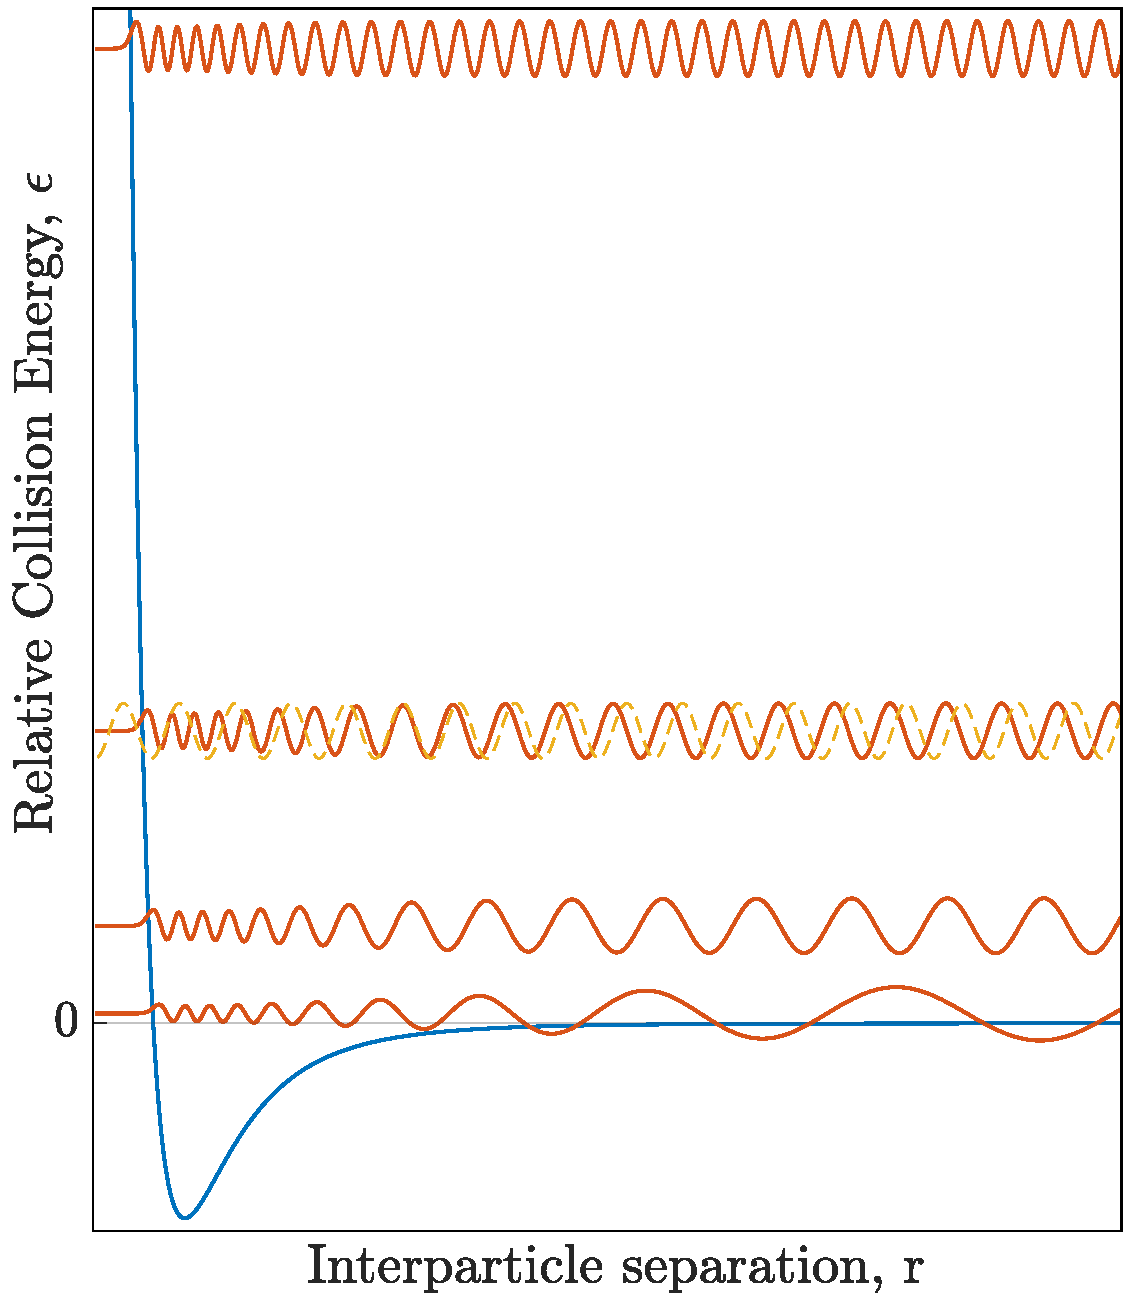
\includegraphics[height=0.6\textheight]{definitionOfStates.pdf}}
	\caption{Examples of scattering state solutions}{Schematic examples of scattering states for several different collision energies undergoing single-channel scattering. At high collision energy the incoming wavefunction is not significantly perturbed by the $\epsilon<0$ part of the potential and simply reflects off the barrier. As collision energy is decreased, the potential begins to effect the incoming wave and results in a compression of the local de Broglie wavelength, $\lambda_{\text{local}} = 2\pi\hbar/\sqrt{2\mu(E-V(r))}$, in the vicinity of the well. Note, the dashed line shown with the middle scattering state is the unscattered wavefunction for comparison. The phase shift, resulting from scattering from the potential, is apparent as $r\,\rightarrow\,\inf$.}
	\label{fig:3collwf}
\end{figure} 

Atomic collision theory separates the scattering interaction into regions that exhibit very different characteristic length and energy scales \cite{Julienne2009a}.
Through this separation, a great deal of insight has led to the development of many practical methods for studying the scattering states and weakly-bound molecular states near zero-energy \cite{wbz99,Gao01,gao04,Bohn1999,Julienne2009a,Vogels1998,Moerdijk1995,Julienne1989}.
In the following, we will outline the critical results of these treatments of atomic collisions.

\subsection{Single channel scattering near threshold} \label{ssec:low_energy}
Consider the collision of two structureless atoms interacting by a single adiabatic Born-Oppenheimer potential, which at long-range is described by a van der Waals potential, $V(r)_{\text{long}} = -\frac{C_6}{r^6}$.
We are interested in understanding the van der Waals interaction as it is the dominant term in the long-range interaction between two ground state neutral atoms.
This potential has a characteristic length, $R_{\mathrm{vdW}} = \frac{1}{2} \left(\frac{2 \mu C_6}{\hbar^2}\right)^{1/4}$, and energy, $E_\mathrm{vdW}=\frac{\hbar^2}{2\mu R_{\mathrm{vdW}}^2}$.
However, the closely related characteristic scales from Gribakin and Flambaum \cite{Boisseau2000a,gfl93} prove to be more useful 
\begin{equation}
	\bar{a} = \frac{4 \pi}{\Gamma(1/4)^2}R_{\mathrm{vdW}} \quad\quad \bar{E}=\frac{\hbar^2}{2\mu\bar{a}^2}
\end{equation}
where $\Gamma(x)$ is the Euler Gamma function.
The wavefunction for the equivalent 1D system describing the radial motion is found by solving the radial Schr\"{o}dinger equation
\begin{equation} \label{eq:3radSE}
	-\frac{\hbar^2}{2 \mu}\frac{d^2 \phi_{\ell}}{dr^2} \left( V(r) + \frac{\hbar^2\ell(\ell+1)}{2\mu r^2} \right) \phi_{\ell}=E\phi_{\ell}
\end{equation}
Solutions of Eq.\,\ref{eq:3radSE}, for energies $E>0$, are scattering states $\phi_{\ell}(E)$ with collision wavevector $k=\sqrt{2\mu E/\hbar^2}$.
In the region $r\gg\bar{a}$, the scattering states approach the free particle states but with the additional phase shift $\eta_\ell$
\begin{equation} \label{eq:3asymwf}
	\phi_{\ell}(E)\,\rightarrow\,\frac{\sin(kR-\pi\ell/2+\eta_{\ell})}{\sqrt{k}}
\end{equation}
with de Broglie wavelength $\lambda = 2\pi/k$.
Fig.\,\ref{fig:longRange} gives an example scattering state for $^{86}$Sr undergoing a collision at $10$\,nK.
Note the significant differences in length-scales between each result despite the range of the interaction being restricted to $<\!100\,\text{a}_0$.
\begin{figure} 
	\centerline{
	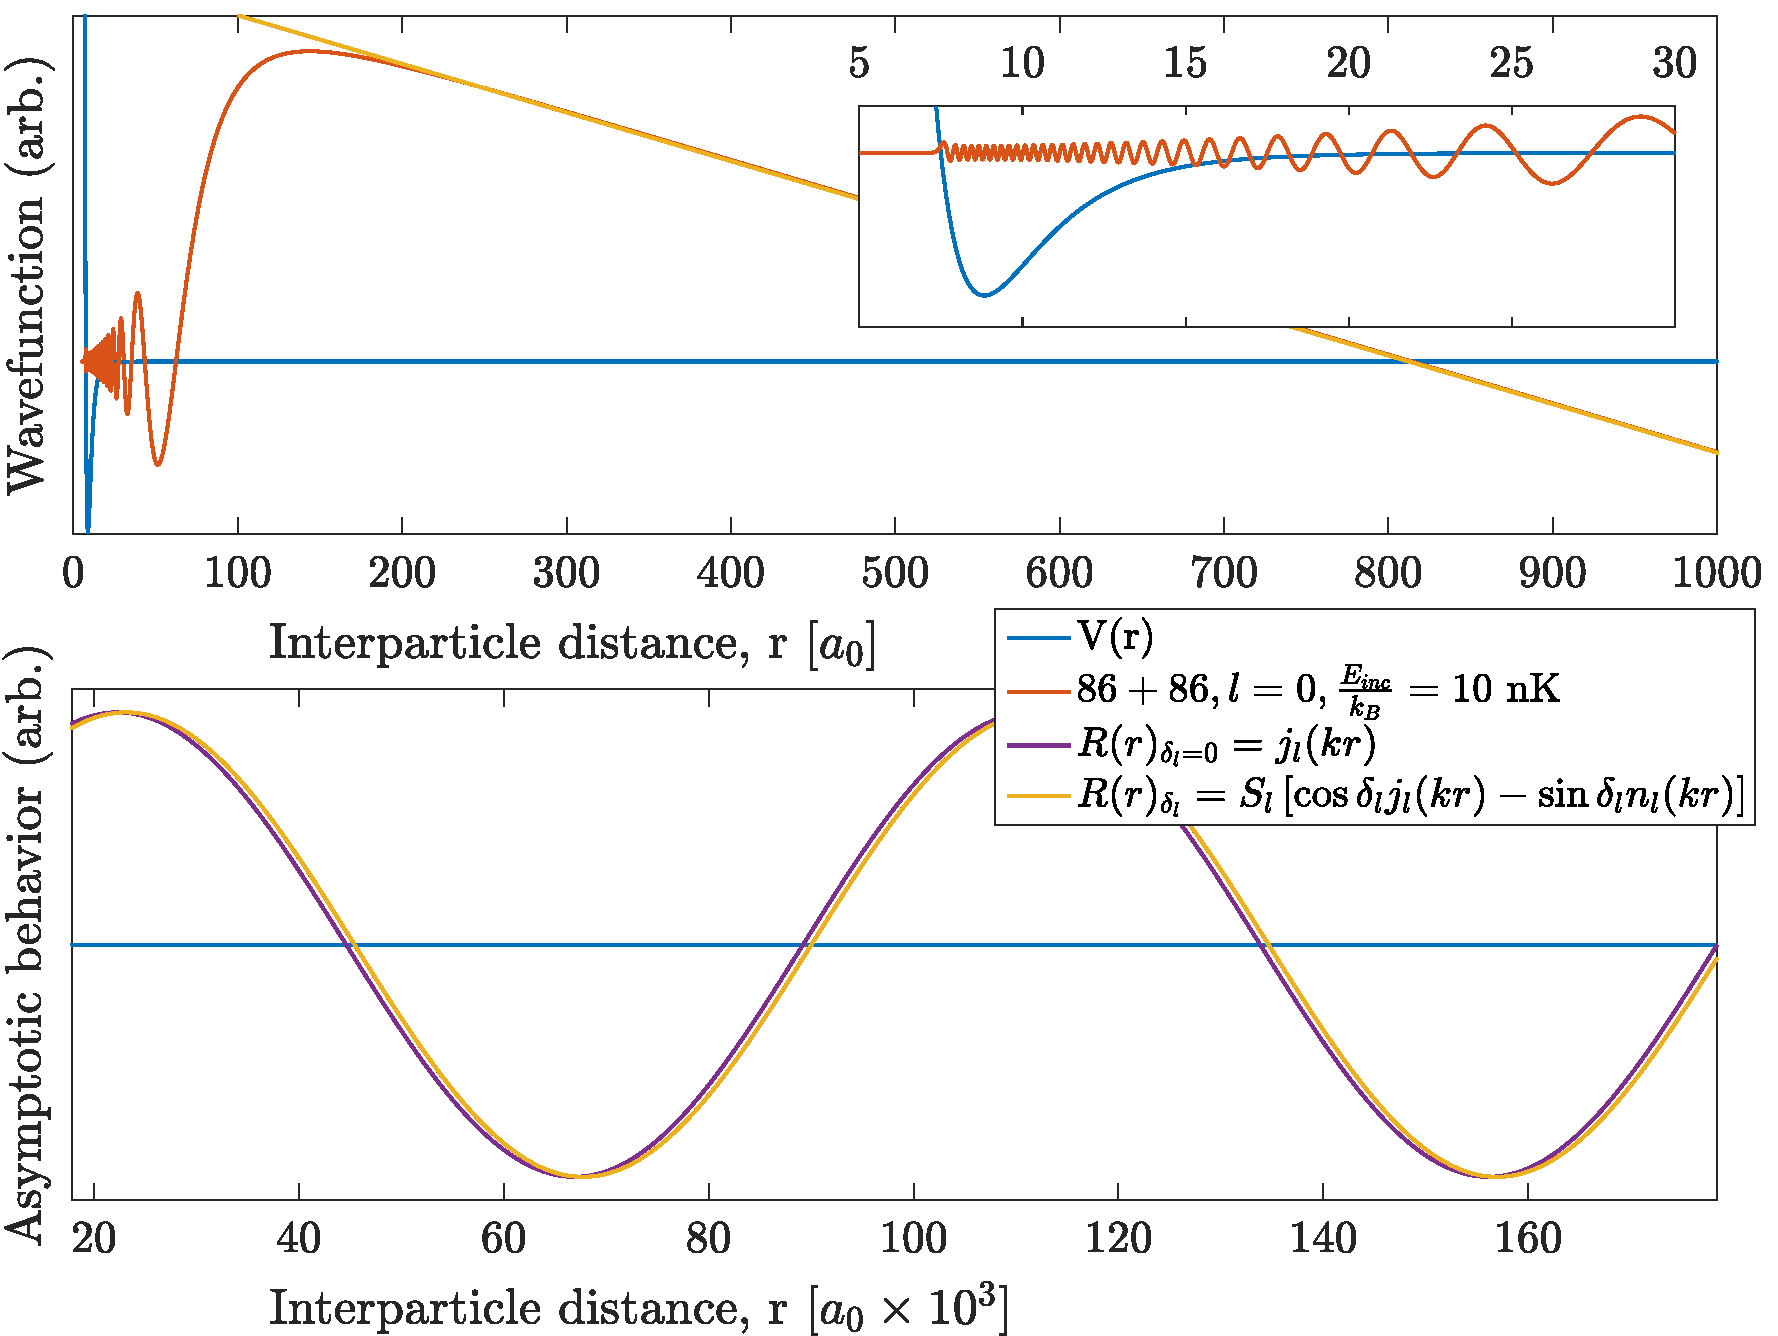
\includegraphics[height=0.6\textheight]{86collWF.pdf}}
	\caption{$^{86}$Sr radial scattering wavefunction near $E=0$}{The radial wavefunction for $\ell=0$ at $E/k_B=10\,$nK for a colliding pair of strontium-86 atoms. The top panel shows the region of the wavefunction near the last node which is related to the $s$-wave scattering length. The inset shows a close up view of the wavefunction in the short-range portion of the X$^1\Sigma_g^+$ ground state potential where the oscillations and amplitude of the wavefunction are strongly effected by the potential. In the asymptotic range, shown in the bottom panel, the scattered wavefunction (red) and the asymptotic free particle state (yellow) are overlapping and shifted with respect to the unscattered free particle wavefunction (purple). Note that the form of the asymptotic wavefunctions given in the legend is equivalent to that given in Eq.\,\ref{eq:3asymwf} \cite{Alexander2014, Sakurai2010}.}
	 \label{fig:longRange}
\end{figure} 

A physical intuition for origin of the phase shift $\eta_{\ell}$ in Eq.\,\ref{eq:3asymwf} may be gained by considering the scattering state $\phi_{\ell}$ for different energies as shown in Fig.\,\ref{fig:3collwf}.
Starting with atoms in the asymptotic region, where the interparticle spacing is large, we see that for atoms approaching one another with low energy, as they near $r\sim\bar{a}$ they begin to be accelerated by the interatomic potential due to increasing potential energy.
This acceleration results in a compression of the local de Broglie wavelength to $\lambda_{\text{local}} = 2\pi\hbar/\sqrt{2\mu(E-V(r))}$ which in turn results in a change of the overall phase of the wavefunction as the scattered state wavelength is pulled inward relative to the unscattered state wavefunction.
In the limit $E\rightarrow0$, $V(R)$ becomes the dominant energy scale such that $E - V(r) \approx V(r)$ and the local de Broglie wavelength becomes independent of the incident energy.
Therefore near threshold, small changes in the relative collision energy do not compress the wavefunction any further in the region $r\lesssim\bar{a}$ and the imparted phase shift, due to acceleration by the potential, is constant.
This is the origin of the $s$-wave scattering length, $a$.
The scattering phase shift may be related to the $s$-wave scattering length $a$ by
\begin{equation}
	a = -\frac{\tan \eta_0(k)}{k}
\end{equation}
where $\eta_{\ell=0}$ is the additional phase in Eq.\,\ref{eq:3asymwf} and $k=\sqrt{2 \mu E/\hbar^2}$ is the collision wavevector.
The value of the $s$-wave scattering length may also be seen as a measure of the peak-to-peak shift between the asymptotic wavefunction and the unscattered wavefunction at long-range as shown in Figs.\,\ref{fig:3collwf} \& \ref{fig:longRange}.
Finally, as energy is increased, the effect of the potential on the scattering state is reduced and the de Broglie wavelength once more remains constant, at a specific energy, for all interatomic distances.
%This is known as the unitarity limit.

From this simple physical picture, we can also understand how changing a particle's mass will effect it's scattering behavior.
Changes to the reduced mass $\mu$ while keeping $V(r)$ fixed, also lead to a change in the local de Broglie wavelength since $\lambda_{\text{local}} = 2\pi\hbar/\sqrt{2\mu(E-V(r))}$ and therefore a change in the $s$-wave scattering length.
This approach of mass-scaling to predict the scattering lengths of various isotopes of many atomic species has been remarkably successful and narrowed the problem of modeling atomic collisions to one of measuring the interaction potential \cite{Julienne2009a}.
Fig.\,\ref{fig:3massScaling} shows the effect of mass-scaling for a selection of strontium isotopic combinations.
\begin{figure} 
	\centerline{
	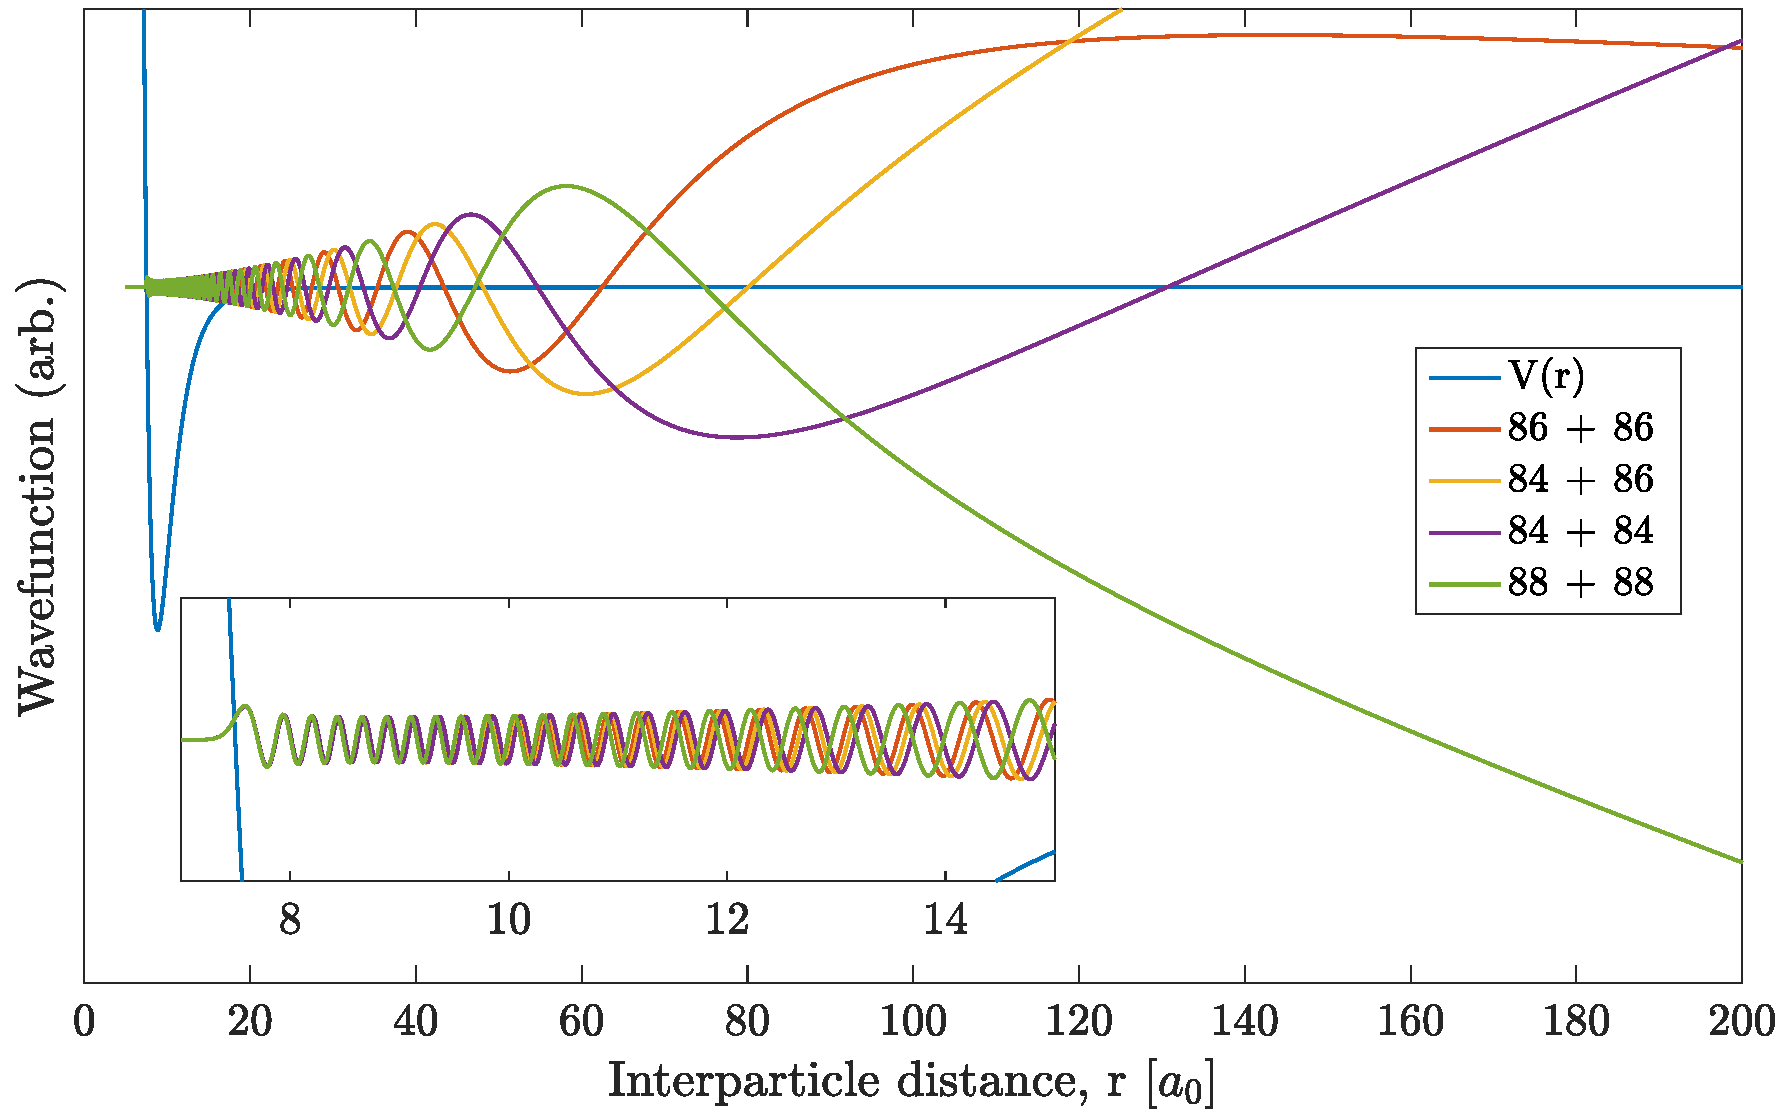
\includegraphics[width=0.7\textwidth]{3massScaling.pdf}}
	\caption{Effects of mass-scaling on strontium scattering wavefunctions}{Varying the reduced mass of the colliding particles leads to vastly different scattering properties between the atoms. From the inset, the wavefunctions start with the same amplitude and phase and quickly begin to oscillate at different frequencies due to the mass differences leading to the large differences in the asymptotic wavefunctions.}
	\label{fig:3massScaling}
\end{figure}  

Moreover, a change in the reduced mass is not isolated to affecting the scattering states.
For bound states, a change in $\mu$ will result in shifting of the binding energies as the solutions to Eq.\,\ref{eq:3radSE} when $E<0$ will also be different.
In some cases this may even lead to changing the number of supported states within the potential well.
Gribakin and Flambaum \cite{gfl93} calculated the relationship between the $s$-wave scattering length and the van der Waals potential to be
\begin{equation}
	a = \bar{a} \left[ 1 - \tan(\Phi - \frac{\pi}{8}) \right]
\end{equation} 
where
\begin{equation}
	\Phi = \int_{R_i}^{\infty} \sqrt{\frac{-2\mu V(R)}{\hbar^2}}
\end{equation}
and $R_i$ is the inner turning point of the potential where $V(R_i)=0$.
The binding energy of the least-bound state of a potential plays an important role in the characterization of scattering from a potential.
In the simplest approximation, the $s$-wave scattering length and the binding energy of the least-bound state are related by
\begin{equation}
	E_{-1} = -\frac{\hbar^2}{2 \mu a^2} \; as \; a\,\rightarrow\,+\infty
\end{equation}
However, accounting for the phase accumulation due to the long-range part of the van der Waals potential modifies the binding energy with $\bar{a}$ \cite{gfl93}.
\begin{equation}
	E_{-1} = -\frac{\hbar^2}{2\mu(a-\bar{a})^2}
\end{equation}
This approaches the universality limit when $a >> \bar{a}$.
Higher-order analytical corrections to the van der Waals potential have also been worked out \cite{gao04}, which relate the binding energy and scattering length through
\begin{equation}
	E_{-1} = -\frac{\hbar^2}{2\mu(a-\bar{a})^2}\left[1 + \frac{g_1 \bar{a}}{a-\bar{a}} + \frac{g_2 \bar{a}^2}{(a-\bar{a})^2}+\dots \right]
\end{equation}
where $g_1=\frac{\Gamma(1/4)^4}{6 \pi^2} - 2$ and $g_2 = \frac{5 g_1^2}{4} - 2$.
Ch.\,\ref{ch:chap5} will employ each of these estimates in analysis of the $^{86}$Sr$_2$ halo molecule.

\addtocontents{toc}{\protect\setcounter{tocdepth}{1}}
\subsection{Remarks on $S$-matrix}
In the previous section, we focused on interactions restricted to a single channel without any decay mechanism.
Such interactions are necessarily elastic as the two-body scattering wavefunction cannot couple outside of its originating channel.
However, most atoms used in laser-cooling exhibit a high degree of internal structure and a quantitative description of their short-range interactions requires consideration of coupling among many different channels.
While a full characterization of such methods is left to Refs.\cite{Nicholson2015a,Hutson2007a,Quemener2012,Chin2010,Alexander2014,Vaillant2014}, here we give the high-level results that will be useful for describing photoassociation in the next section.

In this formalism, atoms are considered to be initially prepared in a single quantum state, which may be characterized by several quantum numbers.
This state is labeled the entrance channel and defined to have energy $E=0$ in the limit $r\rightarrow\infty$.
Scattering channels are specified by a collective set of quantum numbers, $\alpha$, which represents the state of both atoms in the collision.
Channels with $E>0$ are labeled closed, while those with $E<0$ are open.
Upon solving a matrix formulation of the Schr\"{o}dinger equation, the effect of all short-range interactions due to scattering with relative collision energy $E > 0$ is summarized in the unitary $S$-matrix, and reflected in the scattering wavefunctions as $r\rightarrow\infty$. 
Thus the $S$-matrix is the generalization of the energy-dependent phase shift, $\eta_{\ell}(k)$, across all the channels \cite{Julienne2009a}.

In the case of a single open channel scattering near threshold the $S$-matrix is reduced to a single element $S_(k)=e^{2i\eta(k)}$ represented by the complex energy-dependent phase shift $\eta(k)$.
This phase shift also defines a complex energy-dependent scattering length
\begin{equation}
	\alpha(k) = a(k) - i b(k) = -\frac{\tan \eta_0(k)}{k} = \frac{1}{ik} \frac{1-S(k)}{1+S(k)}
\end{equation}
This is an incredibly useful result in the theory of magnetic and optical Feshbach resonances, the latter of which is closely related to photoassociation \cite{Chin2010,Nicholson2015a}.

Finally, the $S$-matrix is related to the elastic and inelastic cross sections by \cite{Pachomov2017}
\begingroup
\addtolength{\jot}{1em}
\begin{align}
	\sigma^{\text{el}}_{\alpha}(k) &= \frac{\pi g_{\alpha}}{k^2} \vert 1 - S_{\alpha \alpha}(k) \vert^2 \\
	\label{eq:sigin}	
	\sigma^{\text{in}}_{\alpha}(k) &= \frac{\pi g_{\alpha}}{k^2} \left( 1 - \vert S_{\alpha \alpha}(k) \vert^2 \right)
\end{align}	
\endgroup
where $g_{\alpha}$ is a channel specific collisional symmetry factor that is equal to $2$ for describing inelastic collisions in a Maxwellian gas of two atoms of the same species in identical spin states \cite{Chin2010}.
\addtocontents{toc}{\protect\setcounter{tocdepth}{2}}


\section{Modeling of photoassociation lineshapes} \label{sec:bohn_and_julienne}
This section develops the theory used to describe one- and two-photon photoassociative spectra with a focus on developing the equations necessary for modeling atomic-loss lineshapes presented in the following chapters.

Recall the classical result for the rate of two-body collisions in a mono-energetic gas is given by $\Gamma = v \,\sigma n = K n$, where $v$ is the velocity of each particle, $\sigma$ is the scattering cross-section, and $n$ is the particle density.
Here $K$ is identified as the two-body collision rate constant, which for inelastic collisions governs the evolution of the density through $\dot{n} = -K n^2$.

Similarly, for scattering of quantum particles, the inelastic collision rate constant\footnote{also called the loss rate constant in literature} for a specific channel $\alpha$, is given by \cite{Nicholson2015a}
\begin{equation} \label{eq:simpleK}
	K^{in}_{\alpha}(k) = v\,\sigma^{in}_{\alpha}(k)
\end{equation}
where $v=\hbar k \mu$ is the relative collision velocity in the center-of-mass frame for the atom pair with reduced mass $\mu$ and $\sigma^{in}_{\alpha}(k)$ is given by Eq.\,\ref{eq:sigin}.
We see that the inelastic cross section simply characterizes the coupling of channel $\alpha$ to all other channels by recalling that the scattering $S$-matrix is unitary and thus
\begin{equation}
	1 - \vert S_{\alpha \alpha} \vert^2 = \sum_{\alpha' \neq \alpha}\vert S_{\alpha \alpha'} \vert^2
\end{equation}

%In general, when several partial waves are needed to describe collisions between particles, then the partial loss rate constants, $K^{in}_{\alpha_i}$, must be summed over each partial wave.
In the case of ultracold photoassociation, we are concerned with the evolution of a single ground state undergoing $s$-wave collisions that is coupled to one or few internal states leading to decay.
Thus, at a fixed collision energy $\epsilon = \hbar^2 k^2 / 2\mu$, the loss rate constant due to inelastic collisions may be written as 
\begin{equation}
	K_{\text{loss}}(k) = g \frac{\pi \hbar}{\mu k} \sum_{\alpha' \neq \alpha}\vert S_{\alpha \alpha'} \vert^2
\end{equation}
Finally, in order to compare to experimental data, we must consider a thermal average of the loss rate constant given by \cite{Julienne2009, Julienne2009a, Krems2009a}
\begin{align} \label{eq:kLoss}
\nonumber
  \langle K \rangle_\text{thermal} &= \int_0^{\infty} d^3\vec{v} f_\text{v,two}(\vec{v})\,|\vec{v}|\,\sigma_{in} \\
  \nonumber
                                  &= \int_0^{\infty} d\epsilon  f_\text{E,two}(\epsilon)\, g \frac{\pi \hbar}{\mu} \frac{\hbar}{\sqrt{2 \mu \epsilon}} \sum_{\alpha' \neq \alpha}\vert S_{\alpha \alpha'} \vert^2 \\
                                  &= \frac{g}{h\,Q_{T}} \int_{0}^{\infty} d\epsilon \sum_{\alpha' \neq \alpha}\vert S_{\alpha \alpha'} \vert^2 \,e^{-\epsilon/k_{B}T}
\end{align}
where $Q_T=\left( \frac{2 \pi k_B T \mu}{h^2} \right)^{3/2}$ is the partition function.
Here we have performed a change of variables using $\epsilon = \mu v^2/2$.
Eq.\,\ref{eq:kLoss} assumes the relative collision energy distribution, $f_\text{E,two}(\epsilon)$, is a Maxwell-Boltzmann distribution.
\begin{equation}
	f_\text{E,two}(\epsilon) = \frac{2}{\sqrt{\pi}} \frac{\sqrt{\epsilon}}{(k_B T)^{3/2}} e^{-\epsilon/k_B T}
\end{equation}
With the expression for $ \langle K \rangle_\text{thermal}$ in Eq.\,\ref{eq:kLoss}, a description of photoassociation reduces to determining the relevant channel couplings and matrix elements needed from the scattering $S$-matrix.
The general approach when evaluating the $S$-matrix for scattering problems involving two or more channels is the coupled-channel method \cite{PhysRevB.38.4688,Krems2009a}.
Alternatively, analytic approximations for $S$ may be found if the scattering problem can be considered in the isolated resonance regime.
The isolated resonance approximation assumes that each molecular bound state is far from any molecular states and can be described by a local strength parameter independent of energy and molecular detuning \cite{Bohn1999, Nicholson2015a}.
Photoassociation is well described by an isolated resonance treatment as specific resonances are targeted and the number of relevant channels is relatively few.
For the case of one- and two-color photoassociation, Bohn and Julienne have derived approximate analytic expressions of the $S$-matrix elements by considering a multi-channel description of resonant scattering and applying an isolated resonance type treatment to approximate the wavefunctions in all channels \cite{Bohn1999, Bohn1996, Julienne2006}.
%applying a quantum defect treatment

One- and two-photon PAS of ultracold atoms may be modeled by first considering the evolution of a local density given by
\begin{equation}
	\dot{n} = - K n^2 - \Gamma_1 n
\end{equation}
where $\Gamma_1$ is the one-body lass rate due to background collisions and $K$ is the two-body loss rate constant.
Integrating over the trapping volume, the evolution of the total number of trapped atoms is then
\begin{equation}\label{eq:number}
   N(t)= \frac{N_0 \rm{e}^{-\Gamma_1 t}}
   		{\displaystyle 1 + \frac{N_0 \langle K \rangle V_2}{\Gamma V_1^2}(1-\rm{e}^{-\Gamma_1 t}) }
\end{equation}
where $N_0$ is the initial number of trapped atoms, $\langle K \rangle$ is an averaged loss rate constant, and $V_q$ is the effective trap volume given by
\begin{equation}\label{eq:effectivevolumes}
	V_{\text{q}}=\int_{\mathrm{V}} d^3\vec{r} \, \exp{-\frac{qU(\mathbf{r})}{k_{B}T}},
\end{equation}
for trapping potential $U(\vec{r})$\footnote{Note that Eq.\,\ref{eq:number} is typically stated with the factor $2 N_0 \langle K \rangle$ in the denominator. This additional factor of $2$ is from the collisional symmetry factor, $g_\alpha$, mentioned previously. In our notation, the value of $\langle K \rangle$ incorporates this additional factor of $2$.}.
A derivation of these trapping volumes is given in App.\,\ref{app:effective_volumes}.

In one-color photoassociation, a single laser at frequency $\omega_1$ couples pairs of colliding ground state atoms with relative kinetic energy $\epsilon$ to an excited bound state $b_1$ with energy $E_{b1}$ and decay rate $\gamma_1$.
Here, $\Delta_1 = \omega_1 - E_{b1}/\hbar$ is used to characterize the single photon detuning from the target state.
Following the approach of Bohn and Julienne \cite{Bohn1999}, the theoretical description of the bound state $b_1$ is modeled as being coupled to an artificial, purely repulsive, potential $a_1$ used to simulate decay from the bound state.
State $b_1$ is then allowed to couple to both the artificial channel and the ground state, while the ground state is defined to only couple to state $b_1$ \footnote{This is discussed near Eq.\,3.1 for one-photon PA scattering matrix in \cite{Bohn1999}}.
Thus the scattering probability $\vert S_{\epsilon, a_1} \vert^2$ is the only relevant $S$-matrix element for describing inelastic loss due to one-photon PAS.
This matrix element characterizes the probability that an atom pair in the ground state with relative collision energy $\epsilon$ scatters into the loss channel $a_1$ and is given by
\begin{equation}
	\vert  S_{\epsilon, a_1} \vert^2 = \frac{\gamma_1 \gamma_s(\epsilon)}{(\Delta_1 + \epsilon/ \hbar)^2 + \left( \frac{\gamma_1 + \gamma_s(\epsilon)}{2} \right)^2}
\end{equation}
where ${\gamma}_{s}(\epsilon)$ is the stimulated width of $b_1$ due to coupling to the initial scattering state by the PAS lasers, which for low energy can be expressed as \cite{ctj06,Borkowski2014a,Pachomov2017,Pachomow2017a}
\begin{equation}\label{3equationstimulatedwidth}
	{\gamma}_{s}(\epsilon) = 2 k \ell_{\text{opt}} \gamma_1,
\end{equation}
Where $k=(2\mu \epsilon)^{1/2}/\hbar$ and the optical length $\ell_{\text{opt}}$ parameterizes the coupling strength between the scattering states and the bound state $b_1$ and is related to the overlap between them.
Plugging $\vert S_{\epsilon, a_1} \vert^2$ into Eq.\,\ref{eq:kLoss} then the thermally averaged loss rate constant for one-photon PA is given by
\begin{equation} \label{eq:onePhotonK}
	\langle K \rangle_\text{thermal} = \frac{g}{h\,Q_{T}} \int_{0}^{\infty} d\epsilon \,e^{-\epsilon/k_{B}T} \frac{\gamma_1 \gamma_s(\epsilon)}{(\Delta_1 + \epsilon/ \hbar)^2 + \left( \frac{\gamma_1 + \gamma_s(\epsilon)}{2} \right)^2} 
\end{equation}

Similarly, two-color photoassociation also considers pairs of colliding atoms undergoing collisions in the presence of light fields.
In this scenario, an additional laser at frequency $\omega_2$ is applied to couple a transition between state $b_1$ and another bound state $b_2$ with energy $E_{b2}$ and decay rate $\gamma_2$.
However, whereas in one-color PAS the frequency $\omega_1$ is swept across the resonant energy of the bound state $b_1$, two-color PAS is commonly performed in the Raman regime with a fixed intermediate state detuning $\Delta_1 = \omega_1 - E_{b1}/\hbar$ from $b_1$.
The two-photon detuning is given by $\Delta_2 = \omega_1 - \omega_2 - E_{b2}/\hbar$.
As before, the bound states $b_1$ and $b_2$ are coupled to artificial loss channels $a_1$ and $a_2$ respectively.
Thus the relevant scattering probabilities for two-color PAS are $\vert S_{\epsilon, a_1} \vert^2$ and $\vert S_{\epsilon, a_2} \vert^2$.
Plugging these into $\langle K \rangle_\text{thermal}$, a formal form of the loss rate constant is specified by
\begin{equation} \label{eq:kLoss2Ph}
  \langle K \rangle_\text{thermal} = \frac{g}{h\,Q_{T}} \int_{0}^{\infty} d\epsilon \left[ \vert S_{\epsilon, a_1} \vert^2 + \vert S_{\epsilon, a_2} \vert^2 \right] \,e^{-\epsilon/k_{B}T}
\end{equation}
where the explicit form of the matrix elements, $S_{\epsilon, a_i}(\epsilon,\gamma_1,\gamma_2,\omega_1,\omega_2,\cdots)$, may be found in equations 4.8 and 4.9 of Ref.\,\cite{Bohn1999}.

Typically, a simplifying assumption is applied to Eq.\,\ref{eq:kLoss2Ph} by considering loss from the state $b_2$ at rate $\gamma_2$ to be negligible on the experimental timescales or in comparison to loss due to scattering from $b_1$.
While this is usually a valid assumption for PAS in alkali systems, it is not necessarily true in alkaline-earth system when using bound states of a narrow intercombination line transition as the two-photon intermediate state.
However, taking $\gamma_2=0$, we recover the standard expressions for two-photon PA with scattering probability \cite{MartinezDeEscobar2008,Jones2006,Napolitano1994,Pachomov2017}.
\begin{equation} \label{eq:twoPhotonSe1}
	\vert  S_{\epsilon, a_1} \vert^2 = \frac{(\Delta_2 + \epsilon/\hbar)^2 \gamma_1 \gamma_s}{
  	\left[ (\Delta_1+\epsilon/\hbar+\delta_1) (\Delta_2+\epsilon/\hbar)-\frac{\Omega_{12}^{2}}{4}\right]^2 + \left[ \frac{\gamma_1 + \gamma_s}{2}\right]^2 (\Delta_2+\epsilon/\hbar)^2}
\end{equation}
which includes a shift of the intermediate state $\Delta_1$ induced by laser 1 and the molecular Rabi frequency between states $b_1$ and $b_2$.
Finally, the thermally averaged loss rate constant simplifies to
\begin{equation} \label{eq:twoPhotonKavg}
	\langle K \rangle_\text{thermal}  = \frac{g}{h\,Q_{T}} \int_{0}^{\infty} d\epsilon \vert  S_{\epsilon, a_1} \vert^2 \,e^{-\epsilon/k_{B}T}
\end{equation}

\subsubsection{PAS near narrow intercombination transitions} \label{sssec:narrow_pa}
In the previous section, Eq.\,\ref{eq:kLoss} was presented with an implicit assumption that the loss rate is dependent only on the relative collision energy distribution.
This is, once again, typically a good approximation for photoassociation with alkali atoms using dipole-allowed transitions, as the consideration of single-particle kinetic energy may be neglected due to the natural width of the transition dominating small shifts due to Doppler effect or photon recoil.
On the other hand, photoassociation to bound states near a narrow intercombination line transitions may exhibit sensitivity to Doppler shifts and photon recoil due to the long-lifetime of the excited molecular state, which will effect the observed photoassociative lineshape \cite{Ciuryo2004, Borkowski2014a, Nicholson2015a, Reschovsky2018, Pachomov2017}.
%The narrow natural transition linewidth, may then be on the order of the Doppler and photon recoil shifts, 

PAS lineshapes utilizing such transitions are described by considering both the center-of-mass momentum of particle pairs in addition to the relative-momentum.
We proceed by considering the individual momentum of each particle using Eq.\,\ref{eq:kLoss} written as a thermal average,
\begin{equation} \label{eq:onePasMom}
	 \langle K \rangle_\text{thermal} = \int_0^{\infty} d^3\vec{p}_1 \int_0^{\infty} d^3\vec{p}_2 \,\frac{2 \pi \hbar^2}{\mu |\vec{p}_1 - \vec{p}_2|} \, f_\text{p,two}( \vec{p}_1, \vec{p}_2 ) \, \vert  S(\vec{p}_1, \vec{p}_2, \omega_1, \omega_2, \cdots) \vert^2  
\end{equation}
Assuming that particle collisions are not correlated, or equivalently, that collisions occur rapidly enough that $\vec{p}_1$ and $\vec{p}_2$ are independent, then the two-particle momentum distribution function, $f_\text{p,two}( \vec{p}_1, \vec{p}_2 )$, is written as the product of two single-particle distributions \cite{Ehrenfest2015,Chliamovitch2017,Brown2008}. 
\begin{equation} \label{eq:3two_particle_prob}
\begin{split}
		 f_\text{p,two}( \vec{p}_1, \vec{p}_2 ) &= f_\text{p,one}( \vec{p}_1 ) f_\text{p,one}( \vec{p}_2 ) \\
		  &= \left(\frac{1}{2 \pi m k_B T}\right)^3 \exp{\frac{-(p_1^2 + p_2^2)}{2 m k_B T}}
\end{split}
\end{equation}
where $m$ is the single-particle mass for a sample at temperature $T$.

Eq.\,\ref{eq:onePasMom} may be reduced to the earlier equations for $\langle K \rangle_\text{thermal}$ by performing a coordinate transform into center-of-mass and relative coordinates and integrating over the center-of-mass, as shown in App.\,\ref{sec:standardDist}.
We will consider a special case of this procedure in Ch.\,\ref{ch:chap5} when discussing the truncation of the single-particle kinetic energy and how this truncation effects the relative collision energy distribution in a trapped gas.

We've taken care to include consideration of the center-of-mass momentum, which is important for describing one-photon intercombination line PAS in strontium.
Although, we emphasize that for the two-photon experiments discussed in this thesis, we are not sensitive to Doppler shifts or photon recoil.
Refs.\,\cite{Ciuryo2004, Borkowski2014a} develop a rigorous extension of the standard Bohn and Julienne theory for one-photon photoassociation near an intercombination line which accounts for Doppler broadening and photon recoil.



%%%%%%%%%%%%%%%%%%%%%%%%%%%%%%%%%%%%%%%%%%%%%%%%%%%%%%%%%%%%%%%%%%%%%%%%%%%%%%%%%%%%%%%%%%%%%%%%%%%%%%%%%%%%%%%%%%%%%%%
%The wavefunction of a low-energy scattering state limits our ability
%Long-range photoassociation is 
%weakly-bound molecules since these give the best overlap.
%
%When an ultracold gas of atoms is produced, the atoms are prepared in specific quantum states, and collisions between the atoms occur with an extremely precisely defined energy close to the E = 0 collision threshold of the interacting atoms, where E denotes energy. 
%This permits extraordinary spectral accuracy in probing near-threshold level positions (order of E/h = 10 kHz accuracy for 1 muK atoms)
%Highest probability of excitation is near the Condon point \hl{citations?}
%
%
%PA lets us get at the complexity of the atom internals
%yield info on atomic collisions
%Consequently, understanding the near-threshold bound and scattering states is essential for understanding the collisions and interactions of ultracold atoms. 
%Understanding collisions is essential to the study of cold atoms.
%
%
%I want the reader to know that PA is concerning the scattering wavefunction, that it comes from the overlap integral of the two wavefunctions because this means that it is sensitive to positions of the nodes and can be used to map out the potentials.

%PAS is naturally described in this model, as the formation of molecules often leads directly to atom loss from the ground state population.

%This has led to a 
%
%%%%%%%%%%%%%%%%%%%%%%%%%%%%%
%%% scattering gives phase shift which effects wavefunction
%%%%%%%%%%%%%%%%%%%%%%%%%%%%%
%
%
%
%
%%%%% Jones 06
%Photoassociation modifies atomic collisions The scattering wave function which describes the collision of two cold atoms at a particular energy and angular momentum has a fixed pattern of nodes. 
%This wave function can be viewed as a standing- wave pattern set up between an incoming wave and the wave reflected by the short-range interatomic potential. 
%As discussed in the previous section, this nodal pattern is directly related to the scattering length for the system and hence to the scattering properties of cold atoms. 
%Any process which changes this standing-wave interference pattern changes the scattering properties of the atoms.
%
%
%
%scattering length represent all the complex physics within the interaction region
%	it effects thermalization through cross sections
%	mean field energy
%	Thus once A is known, all of the long-range be- havior of the wave function is determined. - jones 06


%consider the two-particle system as a single quasi particle
%long range part of this quasi-particle is just the eigenstates of the separate particles themselves (only composed of two parts) 
%but the short range part is going to be determined by some complex physics (new eigenstates, what is the coupling mechanism?)
%		the vdW point is the boundary distance?
%		coupling is due to the interatomic potential, there is at least the long-range part falling off as R6, what are the types of interactions which make up the internal wall?


%%%%%
%In the limit 
%
%
%However, photoassociation results in the creation of bound states using 
%In atomic system, this mean forming a bound state or having some interaction with the atoms around you.
%In the previo
%
%
%Through the manipulation of these applied fields, we have the ability to control the evolution of atomic samples and determine detailed information about the natural 
%
%
%easiest way to explain complex scattering length?
%
%
%%% julienne
%Using the complex the scattering length a-ib to represent the $s$-wave S-matrix Saa = exp [−2ik(a − ib)] in the limit E to 0
%Schrodinger equation also determines the bound states with discrete energies Ei < 0.
%In the special case where a goes to inf, the energy of the last bound $s$-wave state of the system depends only on a nd mu with the universal form
%
%S matrix - defines scattering phases and ampltiudes due to couplings between various open and closed channels
%	S found from the asymptotic solutions
%	S is unitary - makes it easy to define channel coupling
%	The S-matrix is the generalization of the phase shift relation across all the channels. It is what is needed to understand the interactions because the interactions lead to coupling phase shifts which will change the cross section!!! - Julienne CM
%
%if single channel then S reprodcues above results
%if inelastic then get complex scattering length (need better way to segue, Julienne 2014 slide 19 - unitarity argument maybe)
%complex scat
%	Real part is the elastic cross section
%	Imag part if the inelastic
%
%last bound state and low E scatter wf look very similar
%	change bound state -> change scatter wf
%WKB arguement to prove
%	Jones 06 version of WKB
%at low E, WKB can describe the wavefunctions well, see that you get the sqrt(k) from this
%inportant for reflection approx?
%mention sqrt(k)

%scattering length is very sensitive to details of potential
%Determmining a is not so easy because the interatomic potential is not known
%	this was one of the pioneering use for photoassociation
%	
%		
%	
%eta = -ka as k goes to zero
%given by exp(2idel) for S?
%
%\subsection{Multichannel scattering} \label{ssec:multi_chan}
%oh... connect the S matrix formalism to Fano resonance scattering
%
%Everything we discussed was for unstructured particles
%	this is the power of the scattering length
%	
%this would be the end of the story if no coupling
%	you'd find your configuration, describe the potential, solve it, and you're done
%of course this isn't actually the case because the eigenstates of the separate potentials couple to one another.
%Even understanding the natural coupling between coupling between potentials is not easy
%
%address somewhere that these types of problems are generally solved via coupled-channel methods which follow the same recipe for the scattering problem as in the single channel case but does so considering all channels simultaneously through matricies defining potentials and their couplings to one another.
%coupled equations are complicated
%	point out references from Julienne, Mies, Bao, Hutson
%	
%But can match at aymptotic wavefunction again and get a lot of insight
%	
%example: multichannel use to describe atom-diatom coupling
%	mutli-channel model (normal MFR diagram)
%		other potentials are due to different combinations of atoms in hyperfine states
%	these potentials can have different magnetic moments
%		means that addition of a magnetic field can tune them relative to one another
%MFR has been extensively studied and is a common tool used in atomic physics
%	
%scattering resonances are due to off diagonal coupling between bound closed channels and scattering open channels
%	give picture
%hand wavy expalanation is that bringing a bound state close will modify the open channel (potential?)
%	this results in a tweak of the phase shift which results in a change in scattering length
%can describe this as a change in the elastic cross section of the incoming open channel
%in general there is also an inelastic cross section that may contribute if the bound state has a finite lifetime.
%	
%define open and close channels		
%
%Also the Chin '10 review on feshbach resonances
%
%Follow the Nicholson 15 paper method of introing the elastic and inelastic cross sections

%Simple WKB estimation predicts zero-energy bound state as E->0
%	every atom would have infinite scattering length at low energy
%	obviously not the case, GF first to determine analytic corrections due to long-range vdW interaction
%		comes about because of phase contribution from the long-range part
%		
%This is the regime we explored with our work in chapter 5
%	probing a bound state just near the dissociation threshold makes us extremely sensitive to the entire phase of the well


%gives limits on cross sections
%So the limits of cross section are the unitarity limit at incoming energy high enough that the particles only see a delta function and the zero energy scattering length due to the phase shift of the molecular potential.
%	slide 24 (not sure I get the upper bound bit)

%free atoms
%scatering as single-particle state (differnet eigenstate)
%	interaction determined by some gnarly stuff
%From scattering theory we know that the long range behavior is determined by short range physics
%	how do we know this? (the dalibard intro)
%Can we come up with good enough pseudo potentials to describe the short range physics and then solve the schrodinger equation to extract wavefunctions?
%	we want wavefunctions because that is the full characterization
%	we don't know the right eigenbasis for the short range part but we can make some guesses (in particular Hund cases setup eigen states for various possible internal states)
%	Bohn and Julienne theory guessed based on using quantum defect theory
%		this pre-supposes that the bound and free wavefunctions are similar (I forget in what respect) but that the bound ones must go to zero as R->Inf
%If we have some notion of the wf then we can construct matricies which define interactions once we add additional coupling to the scattering problem


%the scattering length as a coupling parameter in length units
%	The mean field energy (I think I had a reference on this)
%	slide 26

%While a full quantum close-coupling calculation is the most complete and rigorous method for analyzing cold quantum scattering problems, useful approximations can be applied to realize relatively more "simple" closed analytic formulas describing photoassociation spectra. 

%This section will cover the theory of lineshapes in PAS.
%
%Somewhere I read about three regimes of PAS as a comparison of relevant energy scales. Should explore that here
%
%Pretty much have everything needed from our previous section.
%Relation of rate constant to cross sections is nice and simple
%		Julienne 14 - slide 21
%These fully coupled-channel models are not straightforward to evaluate.
%	Can make assumption to simplify


%\subsection{One-photon excitation of free to bound transitions} \label{ssec:one_color_pa}
%Can recreate the type of model for MFR in a field dressed approach
%	plot showing photon + potential
%	
%
%	
%ANalytic forms for modeling
%	compare all the forms of K
%		the crazy one from BJ 99
%		the simple one with f(p)
%		nicholson 42
%	
%
%show plot with all the terms defined
%
%give loss rate (will need to have introduced before)
%	define terms
%		gammaStim as overlap
%		gamma as molecular lifetime
%		delta as detuning
%		A as coupling strength
%	
%introduce reflection approximation
%	evaluation of overlap
%	reference BJ 99
%	
%give relative-momentum distribution
%	this results in an asymmetric profile
%	give plot
%	
%Number equation vs. time
% The one-body loss rate, $\Gamma$, is due to background
%collisions and off-resonant scattering from the PA lasers.
%
%segue to narrow lines

%\begin{equation}\label{Kintegral}
%   K=\frac{1}{h\,Q_{T}} \int \vert S(\epsilon,\omega_1,\omega_2,...)\vert^2
%   \,e^{-\epsilon/k_{B}T} \; d\epsilon,
%\end{equation}





%
%quick note on the usage of the relative-momentum distribution
%			usually this is all we care about since the CoM part results in doppler shifts which would be neglible on the energy scales of broad dipole-allowed transtions
%			using narrow intercombinations lines, the photon recoil energy is comparable to the bound state lifetime
%				this means that indivual lorentzians might be shifted (each by a different amount) in addition to the total line shape being asymmetric
%			Integration over both degrees of freedom will be an important discussion in the next chapter as we fit spectra and determine the halo binding energy
%
%ideas of limiting cases that can be explored with PAS \cite{Ciuryo2004}
%
%
%

%\subsection{Extension to two-color spectra} \label{ssec:two_color_pa}
%
%Pretty much the same things
%		
%Show new picture with all the couplings defined
%
%
%Now that we have the theory of PAS covered. 
%
%
%
%
%
%PA loss is described with a local equation for the evolution of the atomic density [Eq.~(\ref{densitydecay})]. Integrating Eq.~(\ref{densitydecay}) over the trap volume yields the time evolution of the number of trapped atoms [Eq.~(\ref{number})]. The effective volumes used throughout this analysis are defined by
%
%for trapping potential $U(\mathbf{r})$. The collision event rate constant can be expressed as a thermal average of the scattering probability for loss, $\vert S(\epsilon,\omega_1,\omega_2,...,\mathbf{r})\vert^2$, over the collision energy $\epsilon$. We also average over the trap volume to allow for the possibility that the scattering probability can vary with position in the trap due to inhomogeneity of laser intensity profiles and the density distribution [Eq.~(\ref{equationKeffective})].
%
%%This yields
%\begin{eqnarray} \label{equationKeffective}
%% \nonumber to remove numbering (before each equation)
%  \langle K \rangle&=& \frac{1}{V_{2}}\int_{\mathrm{V}}
%d^3r \,
%          e^{-\frac{2U(\vec{r})}{k_{B}T}} \nonumber \\
%         &&\times \frac{1}{h\,Q_{T}}
%\int_{0}^{U_{max}-U(r)}d\epsilon \vert S\vert^2
%   \,e^{-\epsilon/k_{B}T}.
%\end{eqnarray}
%%\begin{equation}\label{Kintegral}
%%   K=\frac{1}{h\,Q_{T}} \int \vert S(\epsilon,\omega_1,\omega_2,...)\vert^2
%%   \,e^{-\epsilon/k_{B}T} \; d\epsilon,
%%\end{equation}
%where the partition function is $Q_{T}=\left({2\pi k_{B}T \mu \over
%h^2}\right) ^{3/2}$ for reduced mass $\mu$.
%
%
%Bohn and Julienne \cite{bju96} provide an expression for $\vert S(\epsilon,\omega_1,\omega_2,...)\vert^2$ for a collision on the open channel of two ground state atoms (g) with total energy $\epsilon$ leading to loss-producing decay from the excited state $b_1$ with rate $\gamma_1$. (See Fig.\ \ref{PASDiagram}.) It yields
%\begin{eqnarray}\label{equationSprob}
%  \vert S\vert^2 =   \hspace{2.5in}&&\\
%  {(\Delta_2+\epsilon/\hbar)^2{\gamma}_1{\gamma}_s \over
%  	\left[(\Delta_1+\epsilon/\hbar)(\Delta_2+\epsilon/\hbar)-\frac{\Omega_{12}^{2}}{4}\right]^2+\left[ \frac{\gamma_1+\gamma_s}{2}\right]^2(\Delta_2+		 	\epsilon/\hbar)^2}, &&\nonumber
%\end{eqnarray}
%where all quantities are defined in the main text. For simplicity, we have omitted the light shift of $b_1$ due to coupling to the scattering continuum \cite{bju99}. Equation (\ref{equationSprob}) neglects all light shifts due to the trapping laser. Light shifts due to the photoassociation lasers coupling to states outside our model (Fig.\ \ref{PASDiagram}) are also neglected. The thermal energy is much greater than the zero-point energy for trap motion, $T\gg h\nu_{\text{trap}}/k_B$, so confinement effects are negligible \cite{zbl06}.
%
%%$\Delta_1=\omega_1-E_{b1}/\hbar$ and $\Delta_2=\omega_1-\omega_2-E_{b2}/\hbar$ are the one-photon detuning from state $b_1$ and two-photon detuning from state $b_2$ respectively for initial scattering state with $\epsilon=0$.
%
%%, which is a good approximation for our experiment because the light shift of state 1 is small compared to the detuning $\hbar \Delta_1$,
%and lights shifts of states 0 and 2 are approximately equal and will cancel in the determination of the binding energy of the halo state, $E_2$ \cite{rbm04,rfk87}. Neglecting
%
%%We record spectra by varying $\Delta_2$ at fixed detuning from the intermediate state $\Delta_1$
%
%For the experiments reported here, we maintain significant intermediate-state detuning, $|\Delta_1|\gg |\Omega_{12}|$. Thus we are in a Raman configuration, and near two-photon resonance the expression for the scattering probability for a given initial scattering energy Eq.~(\ref{equationSprob}) can be approximated as a Lorentzian
%\begin{eqnarray}\label{equationSprobLorentzian}
% \vert S\vert^2 \approx {A(\epsilon) \over
% \left(\Delta_2+\epsilon/\hbar-\frac{\Omega_{12}^{2}}{4(\Delta_1+\epsilon/\hbar)}\right)^2+\left[ {\Gamma_L(\epsilon)}/{2}\right]^2},
%\end{eqnarray}
%where $A$ and $\Gamma_L$ are defined in Eqs.\ (\ref{ApproxLorentzianQuantitiesMain}) and (\ref{ApproxLorentzianQuantities-2Main}).
%
%As discussed in the text, we analyze loss spectra using the effective expression, Eq.\ (\ref{equationApproxLorentzian}) to account for possible deviations from the single-channel theory \cite{bju96}.
%
%
%
%
%The one-body loss rate, $\Gamma$, is due to background collisions and off-resonant scattering from the PA lasers.
%
%By integrating this equation over the trap volume, we can obtain the evolution of the total number of trapped atoms
%\begin{equation}\label{number}
%   N(t)={N_0 \rm{e}^{-\Gamma t} \over 1+
%   {2 N_0 \langle K \rangle V_2\over \Gamma V_1^2}(1-\rm{e}^{-\Gamma t})}
%\end{equation}
%
%where $N_0$ is the number of trapped atoms at the beginning of the PAS interaction time. The effective trap volumes $V_q$ are 
%\begin{equation}
%	V_{\text{q}}=\int_{\mathrm{V}} d^3r \, e^{-\frac{qU(\mathbf{r})}{k_{B}T}},
%\end{equation}
%
%for trapping potential $U(\mathbf{r})$. 
%
%$\langle K \rangle$ is the trap-averaged collision event rate constant
%\begin{eqnarray}
%  \langle K \rangle&=& \frac{1}{V_{2}}\int_{\mathrm{V}} d^3r \,e^{-\frac{2U(\mathbf{r})}{k_{B}T}} \nonumber \\
%  &&\times \frac{1}{h\,Q_{T}} \int_{0}^{\epsilon_{\text{max}}({\mathbf{r}})}d\epsilon \vert S\vert^2 \,e^{-\epsilon/k_{B}T},
%\end{eqnarray}
%
%which is itself a thermal average of the scattering probability for loss ($\vert S(\epsilon,\omega_1,\omega_2,...,\mathbf{r})\vert^2$) over the collision energy $\epsilon$, with an energy cutoff $\epsilon_{\text{max}}$ to be discussed momentarily.


%% ARCHIVE
%%%%%%%%%%%%%%%%%%%%%%%%%%%%%%%%%%%%%%%%%%%%%%%%%%%%%
%Think I want to introduce the photoassocation by talking about the collisional wavefunction

%what will that do?

%I want to build up ideas about the FCF and need the wf for that
%	to get qf I have to go back to scattering theory

%ideas of the wavefunction become that basis for how you want to talk about interacting potentials


%
%\begin{figure} \label{fig:FeshbachCartoon}
%	\centerline{
%	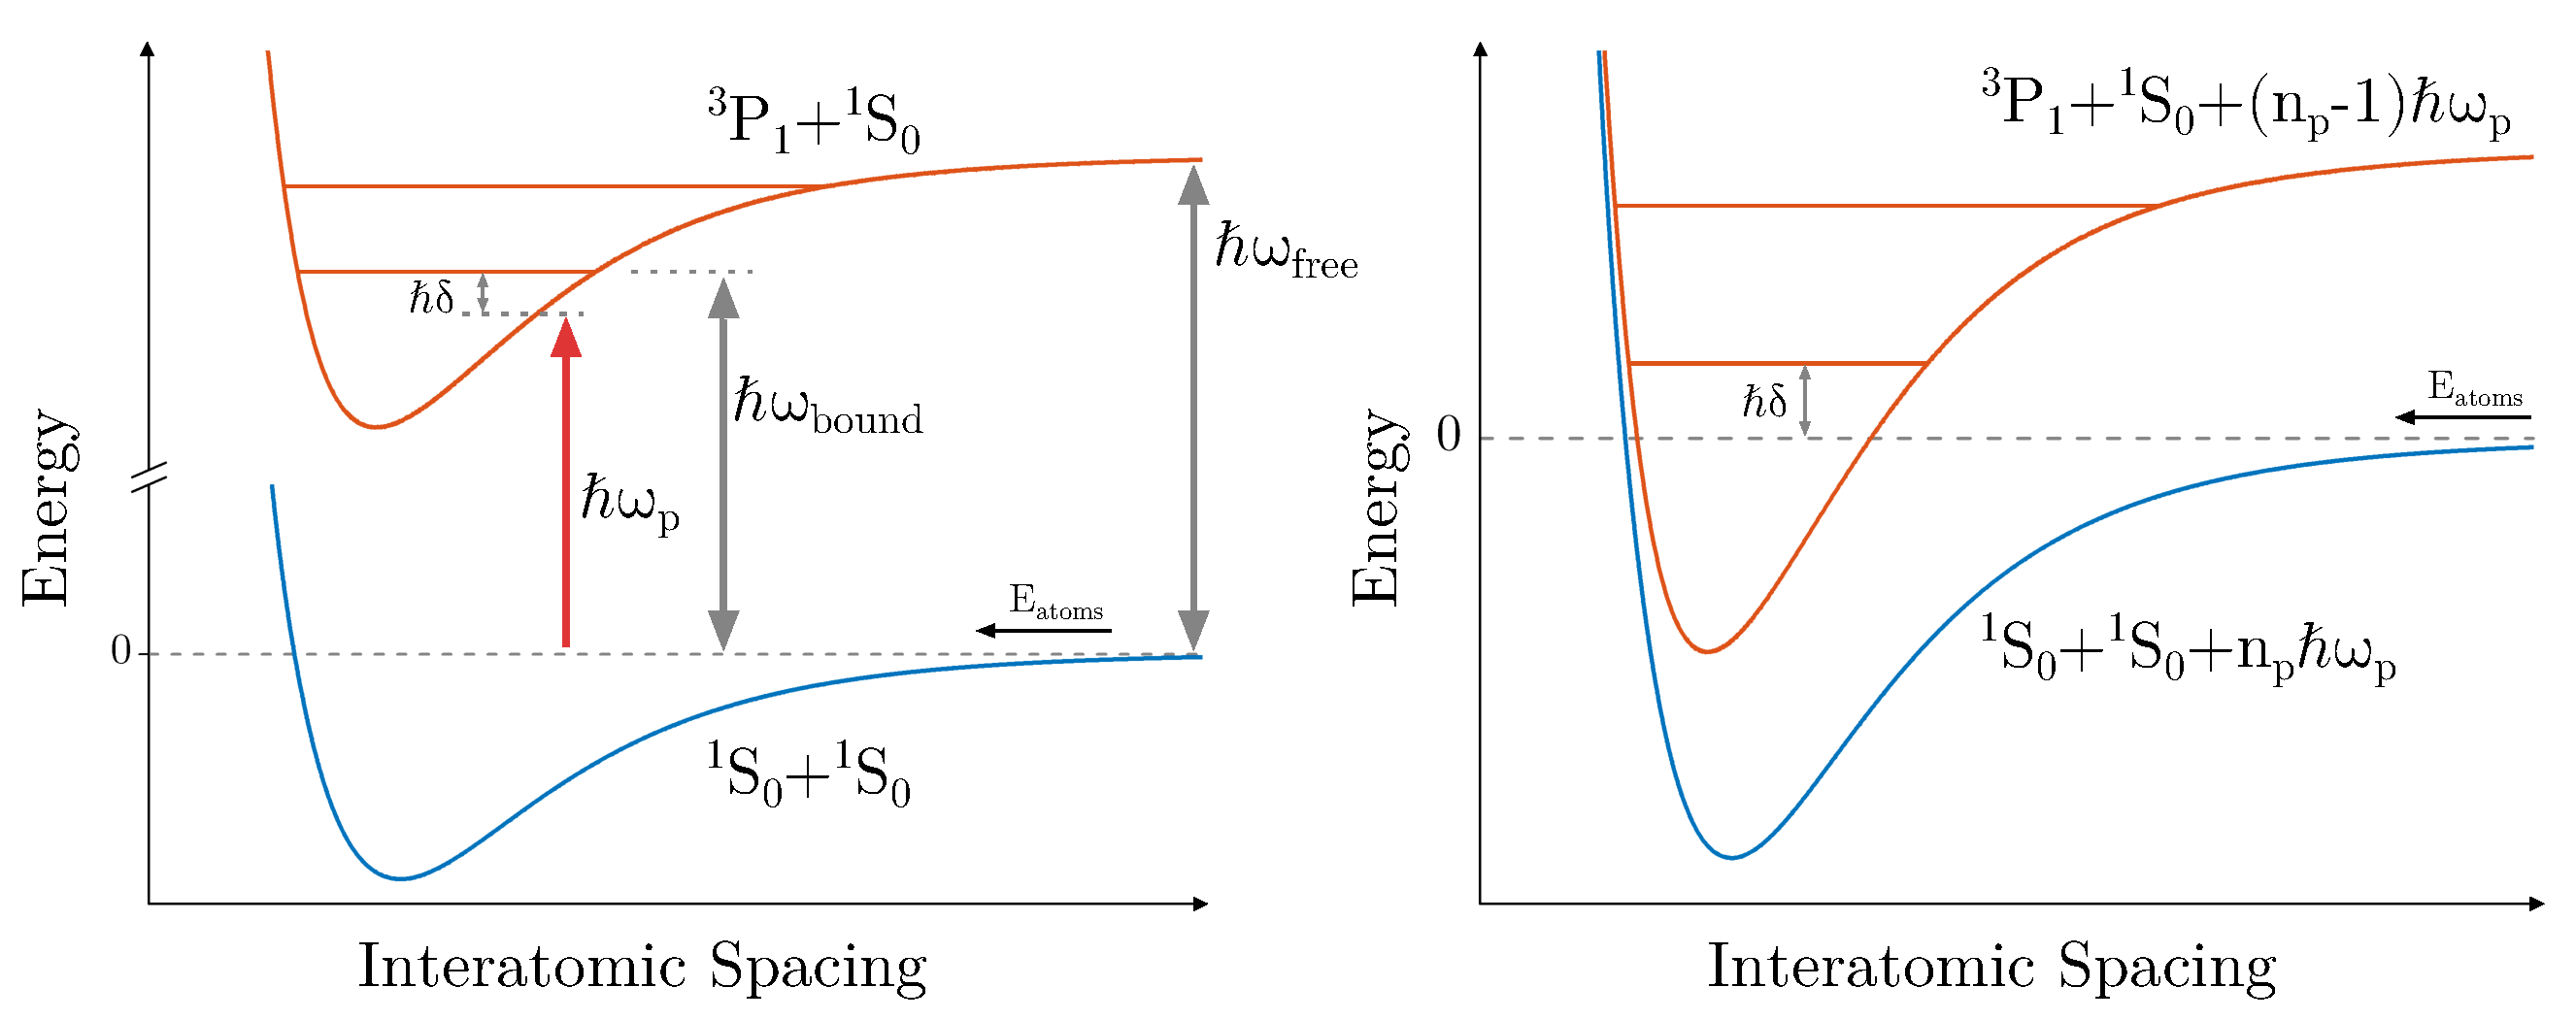
\includegraphics[width=\textwidth]{feshbachCartoon.pdf}}
%	\caption{Schematic representation of a Feshbach resonance}{(a) Potentials for the open ($^1S_0\!+\!^1S_0$) and closed ($^3P_1\!+\!^1S_0$) channel of an optically coupled Feshbach resonance in strontium. (b) The same coupling shown in (a) in the dressed state model. Tuning of the excited potential is achieved by varying the laser frequency detuning, $\delta = \omega_p - \omega_{bound}$, and $\omega_{free}$ is the $^1S_0\!\rightarrow\!^3P_1$ atomic transition frequency.}
%\end{figure} 
%	
%
%The basic idea of a Feshbach resonance is outlined in Fig.\;\ref{fig:FeshbachCartoon}. 
%Consider a simple two channel system, denoted by the open channel and the closed channel. 
%The open channel is generally a ground state potential for two free atoms near threshold. 
%Atoms occupying this state can undergo elastic collisions and, in the absence of any external perturbation, will remain in the open channel. 
%Conversely, the closed channel is a bound state of a higher lying potential who's energy can be tuned relative to the open channel. 
%In the absence of coupling between the states, the open and closed channel remain eigenstates of the system as the tuning parameter, and therefore the energy of the closed channel, is changed. 
%However, in the presence of coupling between the channels, the original eigenstates are mixed and develop an avoided crossing between the bare open and closed channels, when tuned across the resonance. 
%The power of Feshbach resonances comes from the ability to externally manipulate the degree of state mixing, which results in control of the $s$-wave scattering length and the creation of low energy Feshbach molecules.
%
%Magnetic Feshbach resonances (MFR) are used extensively in alkali metal systems to tune the scattering properties of ultracold gases since the ground states of these systems feature a magnetic moment due to an unpaired electron in the valence shell. 
%Thus, MFRs utilize interactions between low lying ground state molecular potentials via spin-dependent couplings. 
%Since both the open and closed channel are ground state potentials, MFRs often exhibit extraordinarily long lifetimes \cite{Chin2010,Kohler2006}. 
%Conversely, in strontium the ground state is a $^1S_0$ state, as shown in Fig.\;\ref{fig:energy_level_diagram}. 
%This state is not magnetically sensitive, so no MFRs exist near the $^1S_0\!+\!^1S_0$ interatomic potential. 
%Fortunately, optical Feshbach resonances (OFR) serve as another method to introduce coupling between the ground state potential (open channel) and a molecular state of an electronically excited potential (closed channel). 
%Our work has utilized coupling between the $^1S_0\!+\!^1S_0$ and  $^3P_1\!+\!^1S_0$ two-body potentials via the narrow $^1S_0\!\rightarrow\!^3P_1$ atomic transition at 689nm. 
%Fig.\;\ref{fig:FeshbachCartoon} shows a schematic of the potentials involved in the OFR of strontium in both the bare atomic and dressed state pictures. 
%In the dressed basis we consider the combined atom + photon field system such that the channels become $\ket{^1S_0\!+\!^1S_0\!+\!n_p\hbar\omega_p}$ as the open channel and $\ket{^3P_1\!+\!^1S_0\!+\!(n_p-1)\hbar\omega_p}$ for the closed channel. 
%As the light field frequency, $\omega_p$, is varied the excited closed channel potential will experience an energy shift relative to the open channel, resulting in resonant coupling between the open and closed channels. \cite{Ciuryo2005,Bohn1997,Fedichev1996a}
%
%The use of a laser field as the coupling scheme in a Feshbach resonance introduces several advantages and complexities that must be considered when determining the expected properties of optical Feshbach molecules. In order to understand these differences, we will briefly outline the key concepts behind Feshbach resonances and the distinctions between optical and magnetic Feshbach resonances.
%
%
%Both MFRs and OFRs can be treated by the same theoretical formalism, as a modification of the collisional properties between two-particles \cite{Nicholson2015a,Chin2010}. 
%
%
%One of the hallmarks of ultracold physics is the simplicity of atomic collisions. 
%
%
%As bosonic atoms get colder they can only collide via $\ell=0$ partial waves and thus the elastic collision rate between two atoms becomes energy independent and can be parameterized by a single fixed quantity, $a_s$. 
%This parameter is known as the $s$-wave scattering length and is determined by the short range molecular potential between two colliding atoms. 


%Through a similar approach, collisions near Feshbach resonances can be modeled by introducing a complex $s$-wave scattering length, $\tilde{\alpha}$. 
%In this model, the magnitude of $\tilde{\alpha}$ influences the elastic scattering rate between particles while the imaginary part describes losses through inelastic scattering. 
%Under an isolated Feshbach resonance model at low energies, this complex scattering length is given by \cite{Chin2010}
%	\begin{equation} \label{eq:complexScatter_constant}
%		\tilde{\alpha} = a - ib = \frac{a_s \Gamma_0}{-E_0 + \imath (\gamma/2)}
%	\end{equation}
%where $E_0$ and $\Gamma_0$ are the energy independent parameters for, respectively, the resonance position and coupling strength between channels, and $\gamma$ is a general decay term associated with loss from the closed channel. 


%Using Eq.\;\ref{eq:complexScatter_constant}, we can note the two main differences between MFRs and OFRs. Most experimentally useful MFRs, such as in Li and K, have negligible closed channel decay, $\gamma = 0$, and a fixed coupling strength between the open and closed channels. 
%Thus, the change in the $s$-wave scattering length takes on a particularly simple form, 
%	\begin{equation} \label{eq:MFRscatter}
%		\tilde{\alpha} = a_s \left( 1- \frac{\Delta}{B - B_0} \right)
%	\end{equation}
%where $B_0$ is the resonance position and the coupling strength is parameterized by a magnetic width $\Delta$, such that $\Gamma_0 = \delta \mu \Delta$ with $\delta \mu$ the difference in magnetic moments between the open and closed channel. 
%
%Conversely, OFRs offer the possibility to tune the coupling strength between the open and closed channel, since the coupling depends on the transition matrix element which varies with the square root of laser intensity.
%Furthermore, since OFRs utilize electronically excited states which have a natural lifetime, $\gamma$ is nonzero. 
%This results in inelastic loss processes for OFRs. Similar to MFRs, we can define the change in scattering length as \cite{Nicholson2015a,Yan2013c,Blatt}
%	\begin{equation} \label{eq:OFRscatter}
%		\tilde{\alpha} = a_s \left( 1 - \frac{w \delta}{\delta^2 + \gamma^2/4} + \frac{i}{2} \frac{w \gamma}{\delta^2 + \gamma^2/4} \right)
%	\end{equation}
%where $\delta=\omega - \omega_0$ is the detuning from the chosen photoassociation resonance at $\omega_0$ as shown in Fig.\;\ref{fig:FeshbachCartoon}, and the width of the resonance is defined by $w = -\ell_{opt} \, \gamma / a_s$. 
%Typically, the strength of OFRs are characterized by their optical length \cite{Nicholson2015a,Chin2010} given by $\ell_{opt} = a_s \Gamma_0 / \gamma = \frac{\lambda_{OFR}^3}{16 \pi c} \frac{ \left| \left< n | E \right> \right|^2}{k} I$. Here $c$ is the speed of light, $\lambda_{OFR}$ is the wavelength of the coupling laser, and $\left| \left< n | E \right> \right|^2$ is the free-bound Frank-Condon factor between the bound state $\bra{n}$ and scattering state $\ket{E}$. 


%Additionally, it is useful to identify the real and imaginary parts of Eq.\;\ref{eq:OFRscatter} as defined in Eq.\;\ref{eq:complexScatter_constant}.
%	\begin{equation} \label{eq:OFRparts}
%		 a_{\scriptscriptstyle OFR} = a_s + \ell_{opt} \gamma \frac{\delta}{\delta^2+\gamma^2/4} \qquad
%		 b_{\scriptscriptstyle OFR} = \frac{\ell_{opt}}{2} \frac{\gamma^2}{\delta^2+\gamma^2/4}
%	\end{equation}
%
%Our previous work exploring the use of an optical Feshbach resonance took advantage of photoassociation transitions with large optical lengths to control the scattering length of an $^{88}$Sr BEC as described by Eq.\;\ref{eq:OFRscatter}. 
%However, all studies of OFR to date have been limited by large atom loss rates \cite{Thalhammer2005,Theis2004,Fatemi2000,Blatt,Yan2013c} which can be modeled as a density evolution, $\dot{n} = -K_{in}n^2$, where $K_{in}$ is the two-body inelastic loss rate constant. 
%In the low energy limit, $k\!\rightarrow\!0$, the inelastic loss rate is given by
%	\begin{equation} \label{eq:K_in}
%		K_{in} = \frac{8 \pi \hbar}{\mu_{r}} b_{\scriptscriptstyle OFR} = \frac{4 \pi \hbar}{\mu_r} \frac{\ell_{opt} \gamma^2}{\delta^2 + \gamma^2 / 4}
%	\end{equation}
%where $\mu_r$ is the reduced mass, $\delta$ is the laser detuning as shown in Fig.\;\ref{fig:FeshbachCartoon}.

%\subsection{Classical} \label{ssec:classical}
%	\begin{figure} 
%	\centerline{
%	  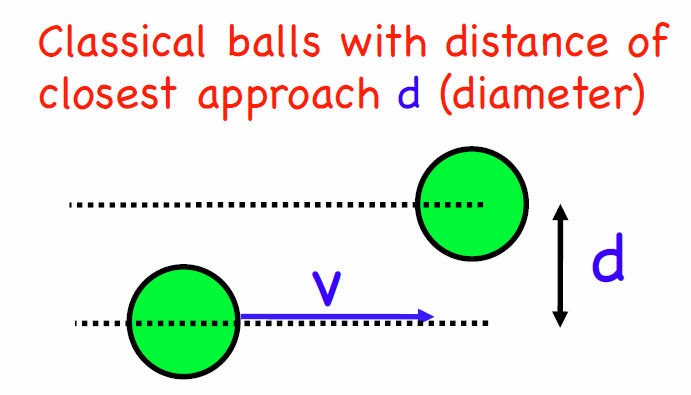
\includegraphics[width=0.5\textwidth]{classicalBalls.PNG}}
%	  \caption{Classical collision}{}
%	  \label{fig:3classical}
%	\end{figure}
%
%Cold atom collisions must be treated quantum mechanically but a some useful information can be determined from classical collisions.
%
%Consider $N$ particles each with radius $d$ and velocity $\vec{v}$ confined to a volume $V$, as shown in Fig.\,\ref{fig:3classical}.
%To determine the rate of collisions imagine freezing all but one of the particles.
%Then in a time $t$, this particle will sweep out a collision volume $V_c = t |\vec{v}| \sigma$ with cross-section $\sigma = \pi d^2$.
%
%
%
%Classically, the number of collisions experienced by a single-particle in a time $t$ for a gas of density $n$ where each particle is moving with velocity $\vec{v}$ is given by $ t |\vec{v}| \sigma n$.
%Thus, the rate of collisions is $\Gamma = |\vec{v}| \sigma n = K n$, with $K = |\vec{v}| \sigma$ the two-body collision rate constant.
%When there is a distribution of relative velocities a sum over contributions from all velocities is required, namely
%\begin{equation}
%	\vert K \vert^2 = \int_0^{\infty}\vec{v}\,f(\vec{v})\sigma d^3\vec{v}
%\end{equation}
%
%
%
%
%hmm.. collisiion in each case
%
%setup coordinates immediately, just say relative 
%
%1. need description of cross section - comes from physical description
%2. description of potential
%
%
%Cross section is a measure of the time between collisions.
%cross sections
%	as a measure of the time between collisions
%	in general energy dependent
%	
%rate coefficient
%	rate from i -> j given by k = sig v
%	when there is a distribution of relative velocities (CM 1.6)
%		dist is normalized
%		maxwell-boltzmann usually the most important
%
%			
%potentials
%	consider how a particle undergoes a collision
%
%
%centrifugal barrier
%	analog - slide 16 Julienne
%	just rxp of particles
